%-------------------------------------------------------%
%                        第2章内容
%-------------------------------------------------------%
\chapter{基于改进MAPPO算法的公交驻站防串车控制方法}\label{第3章}
本章提出一种基于改进多智能体近端策略优化（Multi-Agent Proximal Policy Optimization, MAPPO）
算法的公交驻站防串车协同控制方法。针对传统控制策略在动态公交运行场景中的适应性
不足的问题，通过构建公交运行系统模型，结合异步多智能体强化学习
框架，引入图注意力网络（Graph Attention Network, GAT）与事件图网络（Event Graph Network），
优化多智能体协作机制，旨在实现公交驻站时长的动态调控与全局协调。具体而言，首先基于公交运行
场景特征，建立环形线路的时空状态表征模型，并系统定义强化学习核心要素，包括多维状态空间、
连续动作空间及多目标奖励函数等；其次，设计改进MAPPO算法框架，
利用图结构增强智能体间的信息交互能力；最后，基于强化学习构建闭环控制流程，形成从环境状态映射
到驻站控制策略的完整技术路径。
\section{公交运行系统模型}
\subsection{公交运行环境搭建}
在构建公交运行仿真环境前，需系统分析影响运营稳定性的关键要素，为模型构建奠定基础。
公交时刻表的制定通常依托居民出行需求、路网通行能力、交通流量等多维数据融合分析。
于理想化场景中，若满足以下约束条件：（a）道路资源无竞争性干扰；（b）
司机严格遵循标准化操作流程；（c）站点客流量保持稳定，则公交系统中车辆可维持预期的
车头时距，达到理论最优稳定运行状态。然而现实运营环境中，道路突发拥堵、乘客聚集波动
等随机扰动因素会导致车头时距出现偏差。
因此，需通过动态控制手段优化由此类因素引发的车头时距波动问题。
\begin{table}[htbp]
\centering
\caption{影响公交运行稳定性的因素分析}
\label{tab3-0}
% \begin{tabular}{cp{0.8\textwidth}}
\begin{tabular}{>{\centering\arraybackslash}m{3cm} >{\centering\arraybackslash}m{10cm}}
\toprule
\textbf{影响因素}  & \textbf{对车头时距的影响}\\
\midrule
公交车辆特性 & 车辆的机械性能和司机的驾驶习惯存在差异，每辆车的运行状态不同，导致前后车辆车头时距变化\\
道路交通流状况 & 每辆车发车时间不同，遭遇的交通流状况各异，行驶过程中车头时距会出现不稳定变化 \\
信号交叉口条件 & 每辆车到达信号交叉口时的信号相位情况不同，在信号交叉口的停留时间存在差异，影响车头时距的稳定性 \\
站点客流量 & 站点乘客数量的变化会影响公交车的停留时间，尤其是当某站点乘客数量激增时 \\
\bottomrule
\end{tabular}
\end{table}

影响公交车头时距的因素主要可归纳为以下四个方面，见上表（\ref{tab3-0}）所示。
结合公交系统的实际运行场景和影响因素，公交驻站控制的
运行交互流程可划分为以下环节：

（1）数据动态采集与上传

公交车辆通过车载传感设备实时采集各类运行数据，包括车辆的行驶速度、空间位置、站点停靠时间等关键信息。
所采集数据通过车载通信模块实时上传至综合数据库，通过这种方式实现数据库信息的动态更新，
为后续分析和决策提供最新最准确的数据支持。

（2）控制策略生成与下发

公交调度中心基于实时数据进行深入处理和分析，结合公交系统的运行目标（如准点率、乘客等待时间最小化）、
实时交通状况以及乘客需求等因素，生成动态驻站控制策略。该策略通过专用通信链路实时下发至目标
公交车辆，并同步更新车辆的实时控制信息，以保障车辆运行状态的实时监控。

（3）策略执行与反馈

公交车辆在接收驻站控制指令后，严格按照策略要求执行具体操作，执行完成后，
执行结果通过反馈通道回传至公交系统数据库，基于反馈信息评估策略的实施效果，
以发现潜在问题并及时调整，
从而形成一个完整的闭环管理体系，实现驻站控制的迭代优化。

\subsection{公交环形线路运行模型}
基于上述分析，本文将现实公交系统中的实体（包括公交车辆、公交站点、乘客以及车辆调度中心等）抽象为
数学模型中的基本元素，构建本文的公交运行环境框架。
本章以一条单向环形线路公交系统为研究对象，采用与Daganzo相同的建模思路\cite{daganzo2009headway}，
线路包含$m$个均匀分布的公交站点，运行$n$辆公交车。环形公交线路如图\ref{fig:公交线路与站点示意图}所示。
\begin{figure}[!ht]
    \centering
    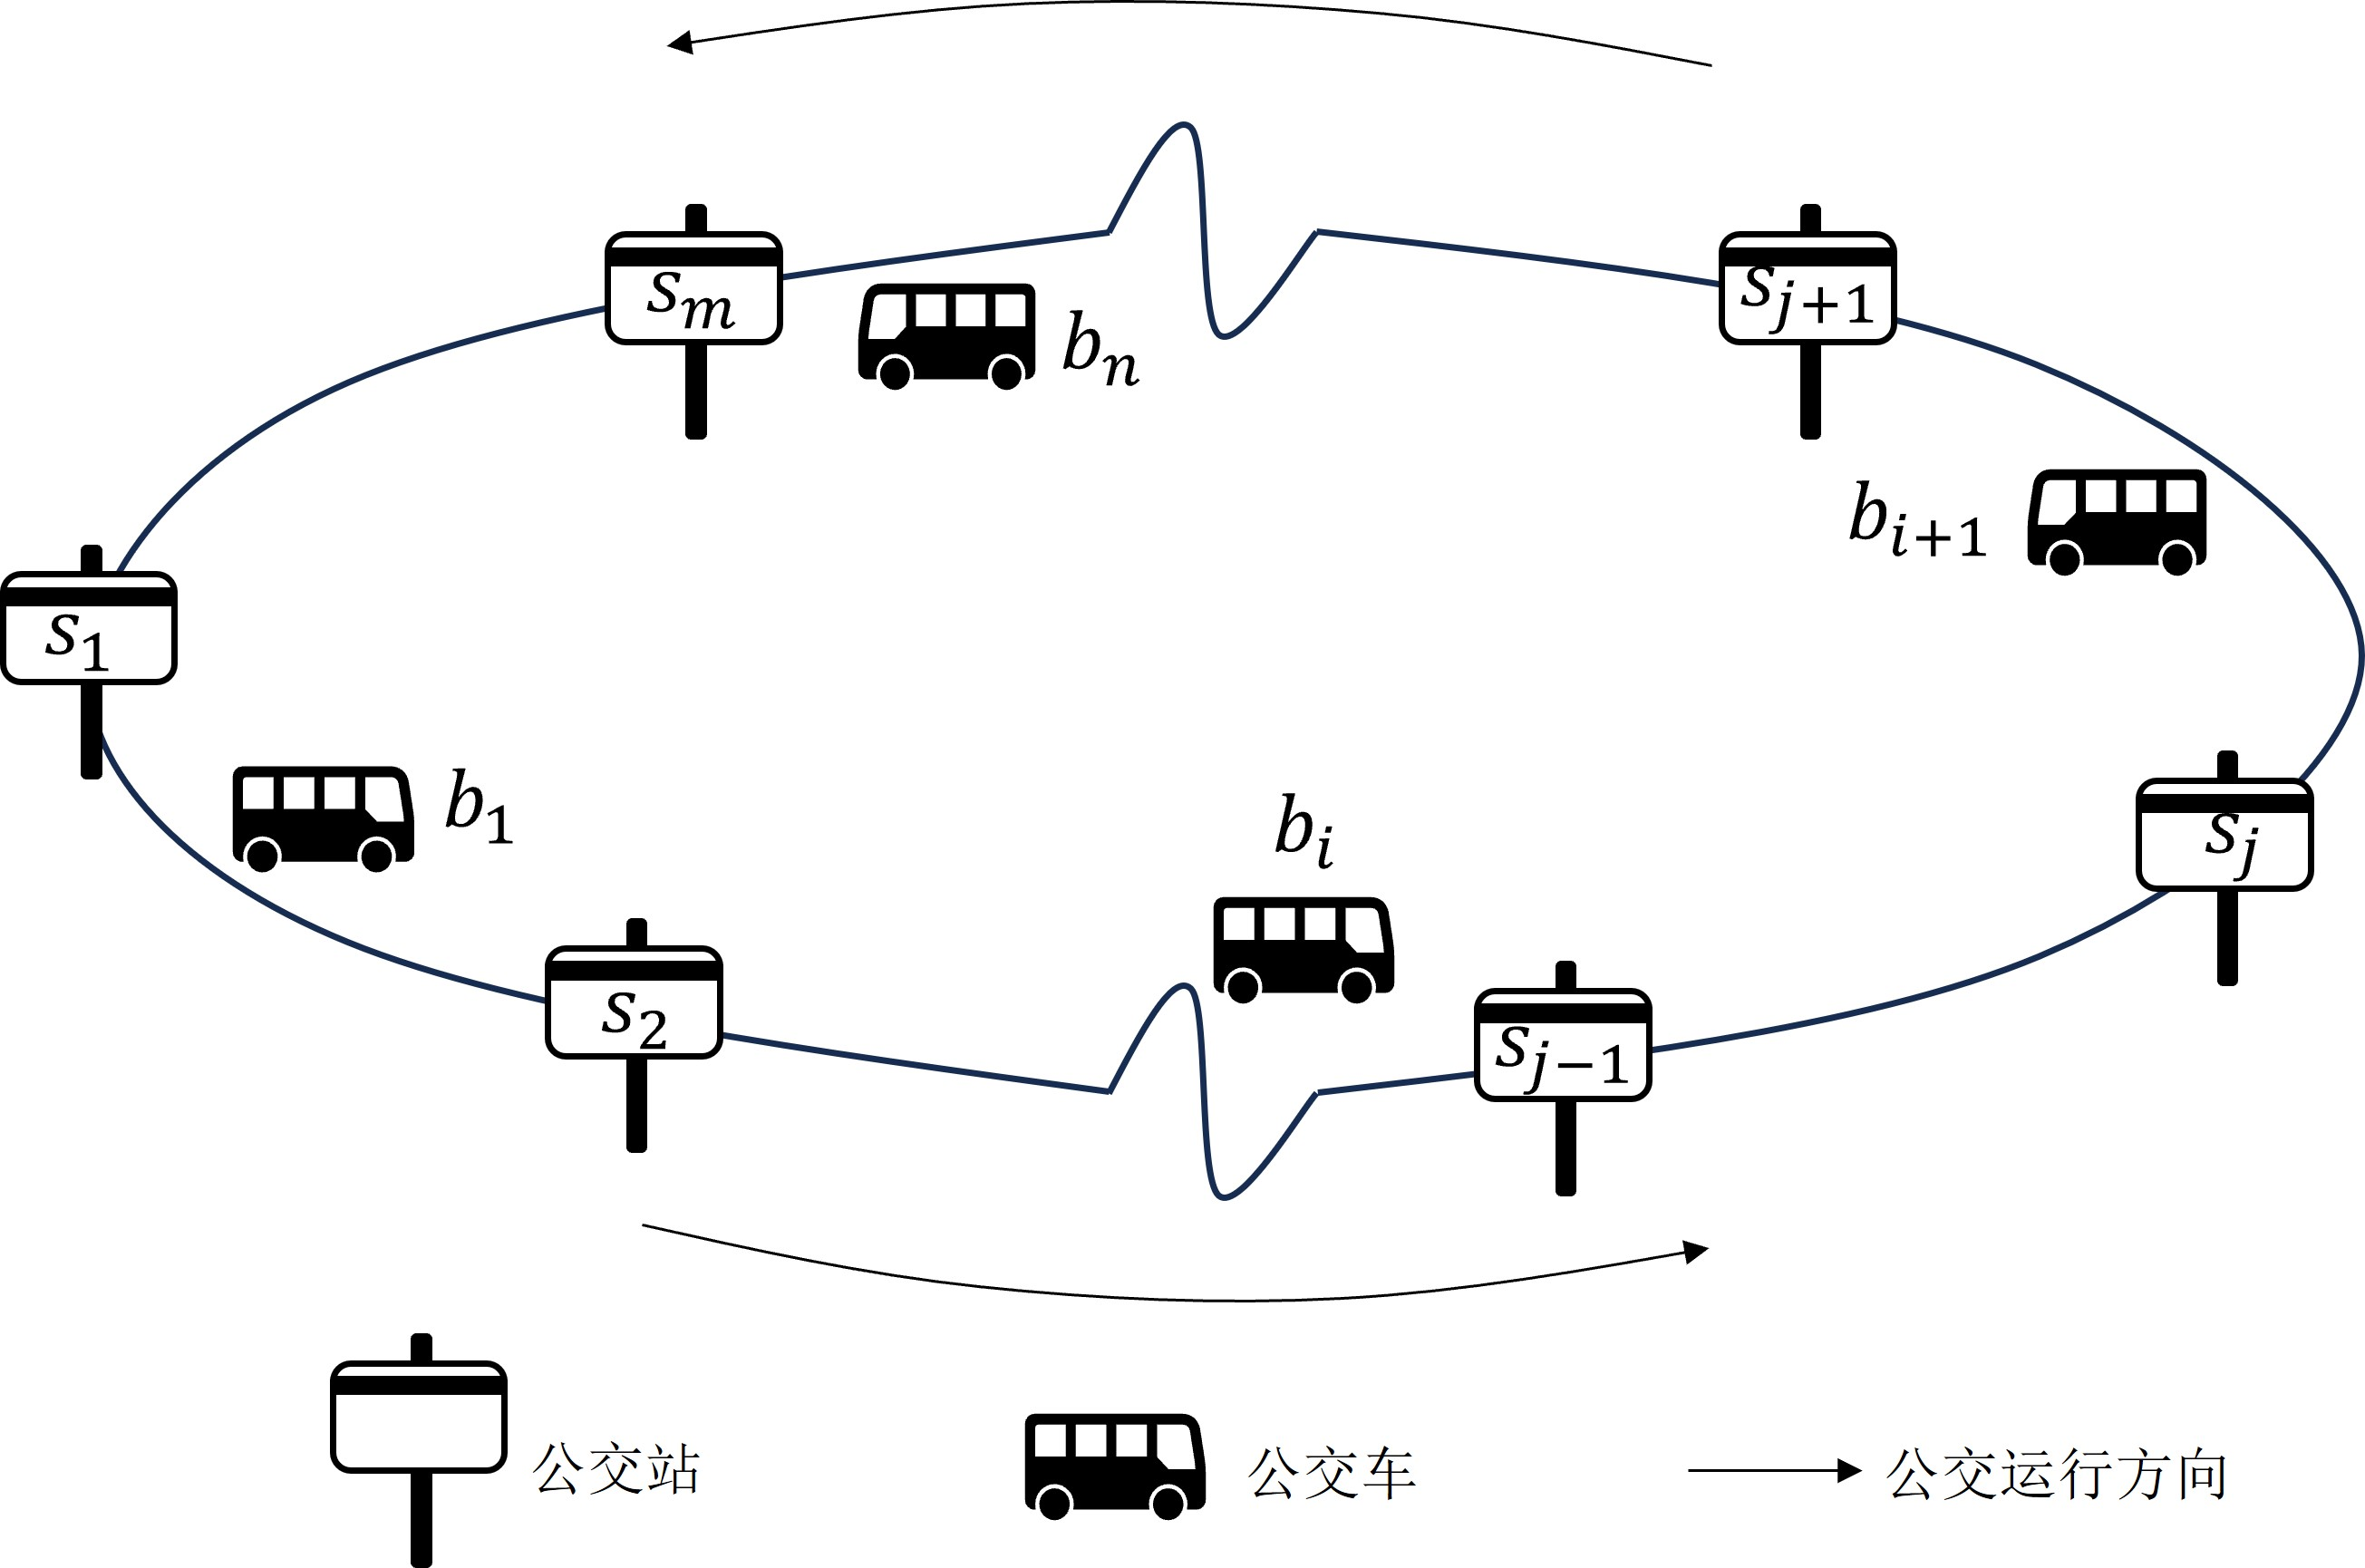
\includegraphics[width=0.59\linewidth]{figures/公交走廊示意图.jpg}
    \caption{公交环形线路示意图}
    \label{fig:公交线路与站点示意图}
\end{figure}

线路上的每辆公交车可以提供多次行程服务，公交车辆以固定的发车间隔$H$按顺序从起始站点出发，
沿线路依次完成下游站点服务，返回起始站点。车辆到达某一公交站时，首先进行站点乘客上下车服务，随后基于实时数据实施驻站控制决策，
完成驻站操作后驶离该站点，前往下一站点服务。
乘客随机到达各站点，车辆抵达相应站点后，乘客按序依次完成上下车操作\cite{刘东2024基于深度强化学习的单线路公交动态驻站控制策略研究}。
所有车辆均具有相同的容量限制。
本文使用的主要符号及其含义如下表\ref{tab3-1}所示。
\begin{table}[!ht]
\centering
\caption{符号和记号列表}
\label{tab3-1}
\begin{tabular}{cp{0.8\textwidth}}
\toprule
\textbf{符号} & \textbf{注释} \\
\midrule
$b_{i}$ & 公交车辆的编号，$i=($1,2,...,$n)$ \\
$s_{j}$ & 公交站点的编号，$j=($1,2,...,$m)$ \\
$ta_{i,j}$ & 公交车辆$i$到达站点$j$的时间 \\
$td_{i,j}$ & 公交车辆$i$离开站点$j$的时间 \\
$A_{i,j}$ & 在站点$j$从车辆$i$下车的乘客数量 \\
$B_{i,j}$ & 在站点$j$登上车辆$i$的乘客数量 \\
$t_{a}$ & 每位乘客下车需要的时间 \\
$t_{b}$ & 每位乘客登上车辆需要的时间 \\
$\lambda_{j}$ & 站点$s_{j}$的乘客到达率 \\
$t_{i,j}$ & 公交车辆$b_{i}$从站点$s_{j-1}$行驶到站点$s_{j}$的实际行驶时间 \\
$\omega_{i,j}$ & 公交车辆$b_{i}$在站点$s_{j}$等待乘客上下车的停留时间，$\omega_{i,j} = \max\{ t_{a}A_{i,j} ,t_{b}B_{i,j}\} $\\
$th_{i,j}$ & 公交车辆$b_{i}$在站点$s_{j}$的驻站时长 \\
$H_0$ & 为满足公交系统需求设计的计划发车间隔\\
$u_{i,j}$ & 在公交站点$s_{j}$等待登上公交车辆$b_{i}$的乘客总需求 \\
$\hat{u}_{i,j}$ & 在公交站点$s_{j}$实际登上公交车辆$b_{i}$的乘客数量 \\
$l_{i,j} $ & 在公交站点$s_{j}$由于容量限制未能登上公交车辆$b_{i}$的乘客数量 \\
$n_{i,j}$ & 在公交车辆$b_{i-1}$和$b_{i}$到达站点$s_{j}$的时间间隔内到达站点$s_{j}$等待登上公交车辆$b_{i}$的乘客数量\\
$U$ & 每辆公交车辆的最大容量限制 \\
$o_{i,j}$ & 公交车辆$b_{i}$离开站点$s_{j}$时的在车乘客数量 \\
$h_{i,j}$ & 公交车辆$b_{i-1}$和$b_{i}$到达站点$s_{j}$的时间间隔\\
$h^-_{i,t}$ & 公交车辆$b_{i}$在$t$时刻与前车的车头时距\\
$h^+_{i,t}$ & 公交车辆$b_{i}$在$t$时刻与后车的车头时距\\
$s_{i,t}$ & 智能体$i$（公交车辆$b_{i}$）在$t$时刻的状态观测\\
$a_{i,t}$ & 智能体$i$（公交车辆$b_{i}$）在$t$时刻到达站点时的控制动作\\
$\triangle d_{i,t} $ & 智能体$i$（公交车辆$b_{i}$）在$t$时刻的驻站时长\\
$\triangle T$ & 公交车辆在单个控制点（公交站点）允许的最大驻站时间\\
$r_{i,t}$ & 智能体$i$（公交车辆$b_{i}$）在$t$执行控制动作后获得的即时奖励\\
% $h^{-}_{i+1,j}$ & 在站点$s_{j}$公交车辆$b_{i}$和$b_{i+1}$之间的后向车头时距\\
\bottomrule
\end{tabular}
\end{table}

基于上述构建的模型，车辆运行轨迹与乘客数量动态变化需遵循如下约束条件：

（1）顺序约束

在该公交系统中，所有的车辆禁止超车，且必须按规定停靠线路上的全部站点，禁止跳站。
车辆队列构成全序关系，
满足车辆$b_{i+1}$始终跟随车辆$b_{i}$（$i$=1,2,...,$n-1$），由于是环形线路，
因此线路上运行的第一辆车
$b_{1}$跟随线路上发出的最后一辆车$b_{n}$。
当公交在$s_{j}$站出现多辆公交车同时抵达的串车现象时，车辆按发车时刻表顺序进站，
即后续车辆必须等待前序车辆完成停靠服务并离站后，才可进入该站点，约束表达式如下：
\begin{equation}\label{顺序约束}
    ta_{i,j} \geq td_{i-1,j} ,\hspace{0.5em} i = 2,...,n; j = 1,2,...,m.
\end{equation}

（2）车辆到站时间

在起始站点$s_{1}$，线路上公交车辆开始第一个循环，车辆$b_{i}$（$i$=1,2,...,$n$）
在起始站点的发车时间即为车辆的到站时间，发车时间$ta_{i,1}$，取决于发车
时间间隔，即:
% 在单向环形线路公交系统中，车辆依次从起始站点（站点$s_{1}$）发车，车辆$b_{i}$
% 在起始点的发车时间$ta_{i,1}$，取决于发车时间间隔，即:
\begin{equation}\label{发车时间间隔}
    ta_{i,1} = (i-1)H,\hspace{0.5em}i = 1,2,...,n.
\end{equation}
% 车辆在起始站点的发车时间也为车辆到达起始站点的时间。

每辆公交车在完成上一次行程前无法开始新的行程，车辆从最后一个
站点$s_{m}$返回始发站$s_{1}$，线路上的公交车在完成一次行程后到达站点$s_{1}$的时间为：
\begin{equation}\label{发车时间间隔}
    ta_{i,1} = td_{i,j} + t_{i,j},\hspace{0.5em} i = 1,2,...,n; j = m.
\end{equation}

车辆从发车站点$s_{1}$离开到达下游站点$s_{j}(j$=2,...,$m)$的到站时间为：
\begin{equation}\label{车辆到达站点的时间}
    ta_{i,j} = td_{i,j-1} + t_{i,j-1},\hspace{0.5em} i = 1,2,...,n; j = 2,...,m.
\end{equation}

（3）车辆离站时间

车辆$b_{i}$到达站点$s_{j}$后需经历以下流程：首先执行停靠服务时长以满足乘客上下车需求；
随后进行驻站决策（该决策逻辑于乘客服务流程完成后激活），根据系统状态确定驻站时间，即
决定车辆在站点的额外停留时间。基于此，
车辆离站时间见下式（\ref{车辆离开站点的时间}）：
\begin{equation}\label{车辆离开站点的时间}
    td_{i,j} = ta_{i,j} + \omega_{i,j} + th_{i,j},\hspace{0.5em} i = 1,2,...,n; j = 1,2,...,m.
\end{equation}

% （4）车辆在站点的停留时间
（4）车辆在站点的服务时间

服务时间是指乘客完成上下车活动所需的时间。由于大多数公交车都有两扇门，
在车乘客的下车过程和在站点等待乘客的上车过程可以同时进行。我们假设
乘客上下车时间遵循乘客数量的线性函数，
则车辆在站点的服务时间取决于所有乘客上下车所用时间中的较大值，
见下式（\ref{车辆在站点的服务时间}）：
\begin{equation}\label{车辆在站点的服务时间}
    \omega_{i,j} = \max \{ t_{a}A_{i,j} ,t_{b}\hat{u}_{i,j}\} ,\hspace{0.5em} i = 1,2,...,n; j = 1,2,...,m.
\end{equation}

（5）站点乘客总需求

在站点$s_{j}$，等待登上公交车辆$b_{i}$的乘客由两部分组成，一部分是由于公交容量限制
未能登上前一辆车的乘客$l_{i-1,j}$，另一部分是相邻两车到达站点$s_{j}$时间间隔内新到达的乘客$n_{i,j}$，
见下式（\ref{站点乘客总需求}）：
\begin{equation}\label{站点乘客总需求}
    \\u_{i,j} = l_{i-1,j} + n_{i,j},\hspace{0.5em} i = 1,2,...,n; j = 1,2,...,m.
\end{equation}

在每个公交站点$s_{j}$，我们假设乘客到达遵循泊松过程，速率为$\lambda_{j}$。
在车辆$b_{i-1}$和$b_{i}$到站时间间隔内新到达的乘客数量是一个随机变量，
且服从泊松分布，如下式（\ref{站间乘客到达数量}）所示。
\begin{equation}\label{站间乘客到达数量}
    \\n_{i,j} \thicksim \mathsf{P} (\lambda_{i,j},h_{i,j}),\hspace{0.5em} i = 1,2,...,n; j = 1,2,...,m，
\end{equation}
\begin{equation}\label{车头时距}
    \\h_{i,j} = ta_{i,j} - ta_{i-1,j},\hspace{0.5em} i = 1,2,...,n; j = 1,2,...,m.
\end{equation}

在站点$s_{j}$等待上车的乘客，其目标下车站点$s_k$的选择服从离散型均匀概率分布，以相同的概率在下游
站点随机选择，见下式（\ref{乘客下车站点}）：
\begin{equation}\label{乘客下车站点}
    s_k \sim \mathcal{U}(s_{(j+\mu) \bmod m} \mid \mu \in \mathbb{N}^+, 1 \leq \mu \leq  m ).
\end{equation}

（6）站点实际上车乘客数量

站点实际上车乘客数量取决于车辆的容量限制$U$、公交到站后
在站点下车的乘客数量$A_{i,j}$以及车上剩余在车乘客数量，在站点$s_{j}$的实际上车人数见
下式（\ref{站点实际上车乘客数量}）：
\begin{equation}\label{站点实际上车乘客数量}
    \\\hat{u}_{i,j} = \min\{ u_{i,j},U-o_{i,j-1}+A_{i,j}\} ,\hspace{0.5em} i = 1,2,...,n; j = 1,2,...,m.
\end{equation}

（7）站点滞留乘客数量

当站点$s_{j}$的候车乘客数量$u_{i,j}$超过车辆$b_{i}$的剩余载客容量时，将触发乘客滞留机制。
我们假设遵循乘客先到先服务（First-In-First-Out, FIFO）原则，根据到达时序部分乘客会被剩余，
等待下一车辆的服务，站点滞留乘客数量如下式（\ref{站点剩余乘客数量}）所示。
\begin{equation}\label{站点剩余乘客数量}
    \\l_{i,j} = u_{i,j} - \hat{u}_{i,j},\hspace{0.5em} i = 1,2,...,n; j = 1,2,...,m.
\end{equation}

（8）在车乘客数量

乘客在车站上下车过程结束后，公交车上的乘客人数会更新。
公交车辆$b_{i}$离开站点$s_{j}$时在车乘客数量为其到站时车上的乘客数量减去下车的
乘客数量加上实际登上车辆的乘客数量，如下式（\ref{在车乘客数量}）所示。
\begin{equation}\label{在车乘客数量}
    \\o_{i,j} = o_{i,j-1}+\hat{u}_{i,j}-A_{i,j},\hspace{0.5em} i = 1,2,...,n; j = 1,2,...,m.
\end{equation}

公交车辆在相邻站点间的行驶过程如下图\ref{fig:公交车辆运行图}所示。
\begin{figure}[!ht]
    \centering
    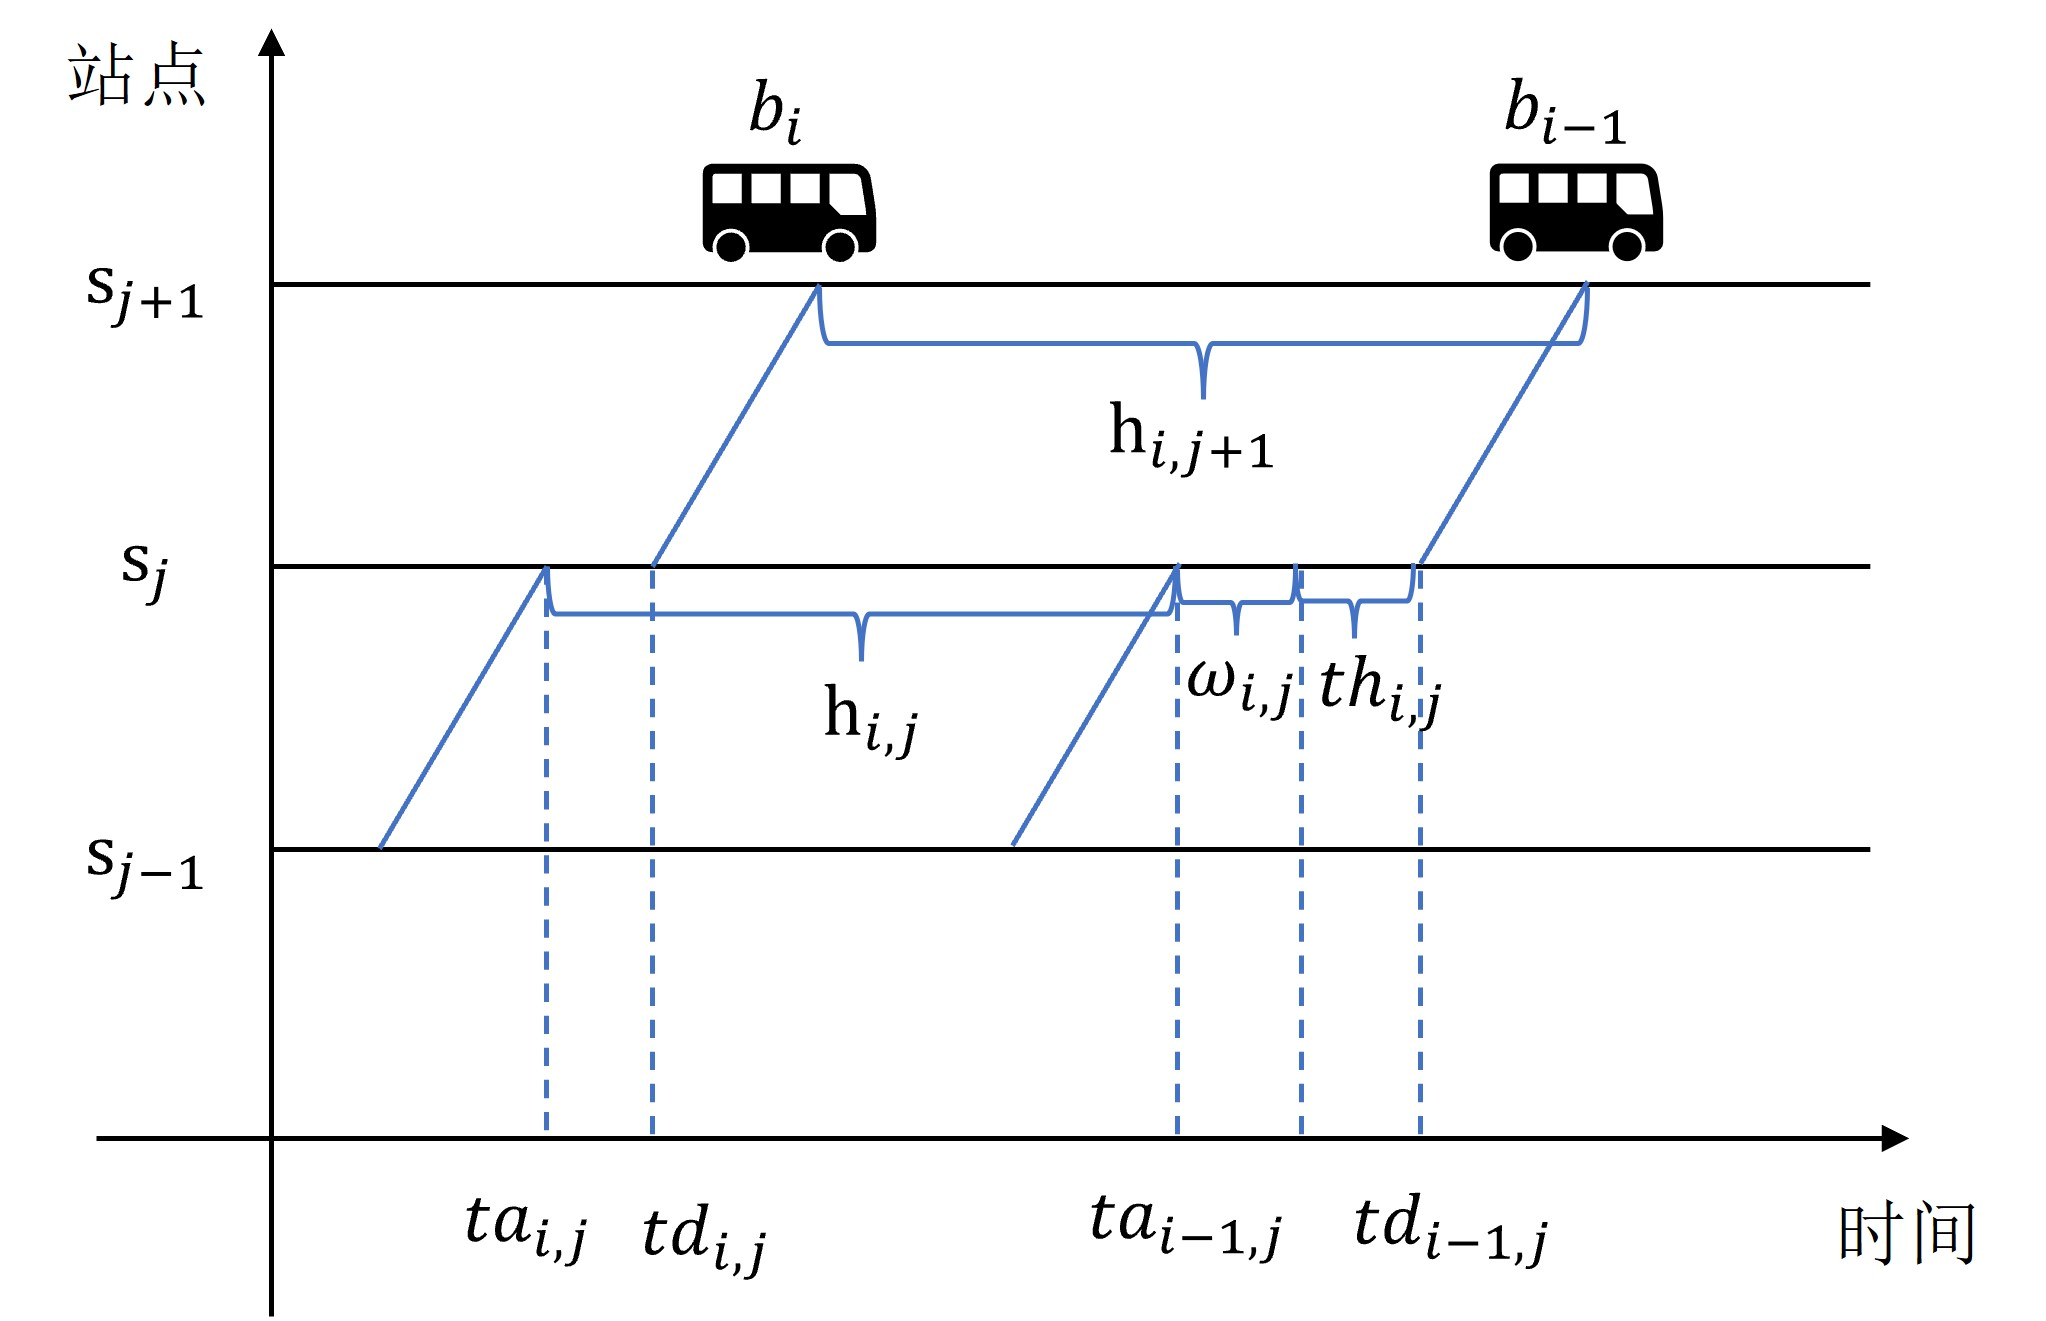
\includegraphics[width=0.7\linewidth]{figures/车辆运行图.jpg}
    \caption{公交车辆运行图}
    \label{fig:公交车辆运行图}
\end{figure}

\section{基于异步多智能体强化学习的公交驻站控制建模}
基于上文构建的公交系统模型，提出深度强化学习框架，将单向环形线路公交车队实时驻站控制
问题建模为异步多智能体强化学习问题。
驻站控制策略在缓解公交串车问题中被广泛采用，在日常车辆的运行过程中可保持车头时距的稳定。
本研究将公交驻站作为多智能体强化学习的控制策略进行建模，以提升公交系统
整体的运营效率。

本研究将公交系统中运行的全部公交车辆视为智能体，并按照发车
顺序对车辆编号。由于公交驻站控制仅发生于公交站点，且公交系统同一线路的所有车辆
不可能同时抵达站点，因此公交系统的中车辆的驻站控制呈现异步特性。
本研究在多智能体强化学习任务中考虑了公交的异步到站特性。
线路上公交车辆驻站控制异步特征如下图\ref{fig:公交到站的异步特性}所示。
\begin{figure}[!ht]
    \centering
    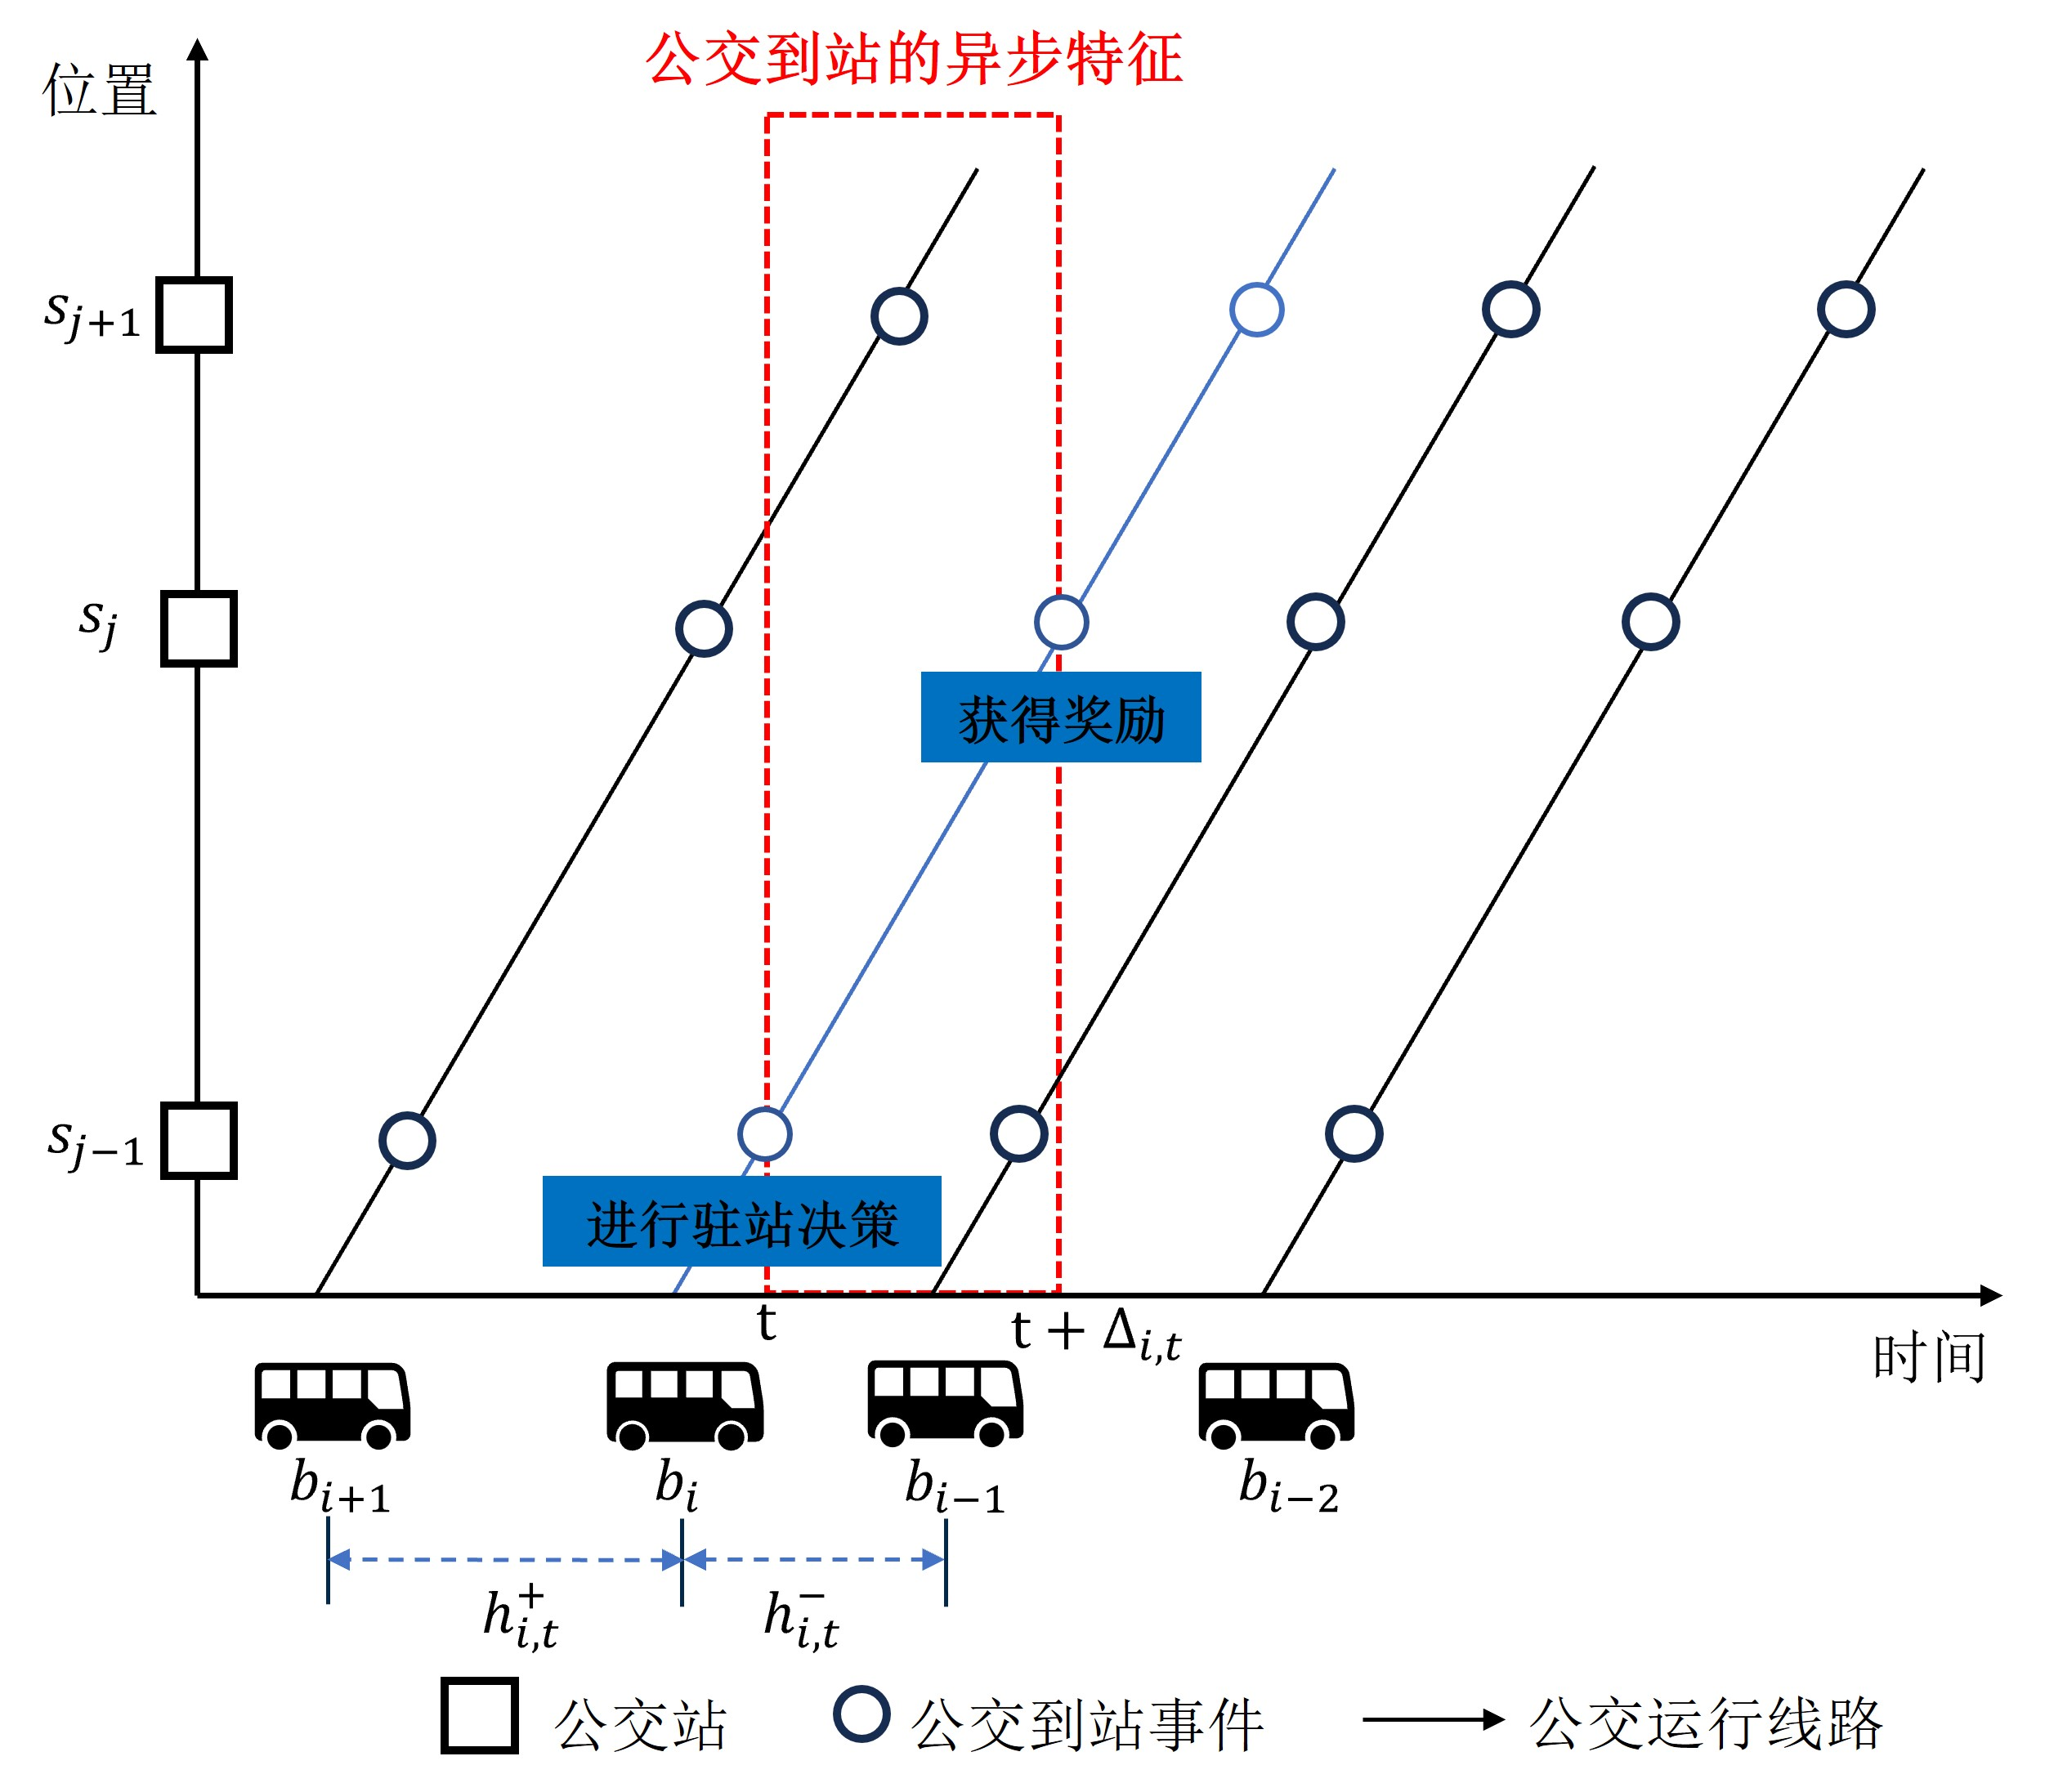
\includegraphics[width=0.51\linewidth]{figures/公交到站的异步特性.jpg}
    \caption{公交车辆驻站控制的异步特性}
    \label{fig:公交到站的异步特性}
\end{figure}

在所述多智能体强化学习的公交驻站控制模型中，每个智能体（每辆公交车$b_i$）在抵达站点$s_j$（控制点）时
执行驻站时长决策动作$a_{i,t}$，当到达下一个站点$s_{j+1}$时获得该动作的即时奖励信号$r_{i,t}$，
这种序贯决策过程被称为马尔可夫决策过程（Markov Decision Process, MDP）。


马尔可夫博弈\cite{shapley1953stochastic}（Markov Game, MG）是马尔可夫决策过程（MDP）在多智能体环境中的扩展，
在公交驻站控制的多智能体强化学习场景中，智能体（公交车辆）的博弈性质主要体现为
动态合作博弈，博弈的核心来源：

（1）车头时距的动态协调：公交车辆的驻站时长直接影响相邻车辆的到站时间间隔（车头时距），
后车需根据前车行为的影响调整自身策略，若前有车较长的驻站时长，可能导致后车被迫延长驻站时间以维持车距的稳定，形成策略链式反应，这种相互依赖的决策过程需要智能体通过博弈平衡个体目标（减少自身延误）与全局目标（系统稳定性）；

（2）乘客需求的间接分配博弈：驻站时长会影响后续站点乘客的累积，车辆通过驻站时长间接争夺乘客资源的“服务权”，行成非零和博弈（一方的收益未必是另一方的损失）；

（3）不完全信息博弈：车辆无法实时获取其他车辆的完整决策信息，仅能基于局部观测调整策略。

基于该博弈论模型，本文将公交线路上车辆协同驻站控制构建为马尔可夫博弈（Markov Game, MG），
其形式化定义见前文式（\ref{式25}）。
将公交系统中全部$n$辆公交车建模为同构智能体，共享相同的状态空间$\mathcal{S}$、
动作空间$\mathcal{A}$及奖励函数$r_{i,t}$。该多智能体强化学习系统的核心建模要素定义见下文所述。

\subsection{状态空间}
在公交系统中，每个智能体$i$（公交车辆$b_i$）的决策过程基于局部可观测状态$s_{i,t}$ ，其包括两部分信息：一部分是能够反映与前后车辆的相对位置关系的信息，
另一部分是与乘客数量有关的信息，可以让智能体实时监测车内载客情况。智能体$b_{i}$
在$t$时刻到达站点$s_{j}$的状态空间信息$s_{i,t}$由前向车头时距$h^-_{i,t}$（公交车辆$b_{i}$
在$t$时刻与前车$b_{i-1}$的车头时距）、
后向车头时距$h^+_{i,t}$（公交车辆$b_{i}$在$t$时刻与后车$b_{i+1}$的车后时距）以及公交在车
乘客数量$o_{i,j}$三部分组成，用元组表示为：
\begin{equation}\label{状态空间}
    \\s_{i,t} = (h^-_{i,t},h^+_{i,t},o_{i,j}/Z),
\end{equation}
其中$Z$为归一化常数。在实际的应用中，可以通过自动车辆定位（Automatic Vehicle Location, AVL）系统和
自动乘客计数（Automatic Passenger Counting, APC）系统等获取所需要的实时信息数据。

\subsection{动作空间}
在所述多智能体强化学习的公交驻站控制模型框架中，智能体$i$（公交车辆$b_i$）在完成站点$s_{j}$的乘客上下车
服务后，触发驻站控制决策机制，生成公交在相应站点的驻站时长，
公交车辆$b_{i}$在$t$时刻到达站点时的控制动作$a_{i,t}$可以表示为下式：
\begin{equation}\label{动作}
    \\a_{i,t} \in [0,1],
\end{equation}
$a_{i,t}$表示为一个0到1之间的连续变量，连续动作空间的设计
可以为智能体提供更丰富的策略选择，允许智能体在无限精细的范围内选择动作，有效克服离散动作空间
存在的量子化误差问题，同时连续动作空间支持基于梯度的策略
优化算法实现驻站时长的微调，可以在一定空间内探索接近最优的策略。

公交在站点的驻站时长表示为：
\begin{equation}\label{驻站时长}
    \\\triangle d_{i,t} = a_{i,t}\triangle T,
\end{equation}
其中$\triangle T$表示公交在站点单次驻站允许的最大驻站时长，用于限制在单控制点的最大驻站
时长，防止过度控制干预。

\subsection{奖励函数}
奖励函数的设计对于智能体学习最优控制动作至关重要。现有关于公交驻站控制的强化学习研究通常将实际
车头时距与计划值的偏差作为奖励构建基础，
同时通过引入控制动作$a_{i,t}$作为惩罚项抑制过度驻站控制干预\cite{alesiani2018reinforcement,wang2020dynamic,wang2021reducing}，
然而此类奖励函数的设计忽略了驻扎控制对乘客出行体验的直接影响，驻站产生的额外等待时间
会显著增加乘客总的出行时间成本。
% 同时考虑到驻站控制对乘客的影响，

本文借鉴Bartholdi等人\cite{bartholdi2012self}提出的公交自组织控制理论，
采用车头时距离散度作为公交系统运行稳定性的度量指标，在奖励函数中引入了
变异系数平方$CV^2$\cite{national2013transit}来构建车头时距偏差项，
同时创新性的将乘客等待时间成本纳入奖励函数，通过引入双重优化目标实现公交
系统稳定性与运行效率的协同提升。这种设计即保留了现有方法通过同时减少
车头时距的均值和方差实现对串车现象的
抑制作用，又通过显性成本约束避免了过度控制干预。本研究设计的奖励函数具体形式如下：
% \begin{equation}\label{奖励函数}
% \begin{aligned}
%     & r_{i,t} = -\omega_1\times CV^2 -\omega_2 T^w_{i},\\
%     & CV^2 = Var[h]/E^2[h],\\
%     & T^w_{i} = T^{w1}_{i} +T^{w2}_{i},
% \end{aligned}
% \end{equation}
% $CV^2$用来量化车头时距的偏差，当车辆按照预先设定的时刻表发车时，期望车头时距$E[h]$可视为一个常数，
% 因此变异系数平方$CV^2$主要由车头时距方差$Var[h]$决定，$CV^2$值越小，表明线路上公交车头时距的偏差越小。
% 乘客总等待时间$T^W_{i}$由两部分构成：站点初始等待时间$T^{w1}_{i}$（乘客到达站点后至首辆公交到站的等待时间）
% 与车内额外延误时间$ T^{w2}_{i}$（因公交实施驻站控制导致车内乘客增加的等待时间）。
% 权重参数$\omega_1$和$\omega_2$（$\omega_1,\omega_2 \in [0,1]  $）用于权衡车头时距均衡性与乘客等待时间的相对重要性。
\begin{equation}\label{奖励函数}
    \\r_{i,t} = -\omega_1\times CV^2 -\omega_2 T^w_{i},
\end{equation}

\begin{itemize}
    \item $ CV^2 = Var[h]/E^2[h]$，用来量化车头时距的偏差
\end{itemize}

当车辆按照预先设定的时刻表发车时，
期望车头时距$E[h]$可视为一个常数，因此变异系数平方$CV^2$主要由车头时距方差$Var[h]$决定，
$CV^2$值越小，表明线路上公交车头时距的偏差越小。

\begin{itemize}
    \item $T^w_{i} = T^{w1}_{i} +T^{w2}_{i} $，乘客总的等待时间
\end{itemize}

乘客总等待时间$T^W_{i}$由两部分构成：站点初始等待时间$T^{w1}_{i}$（乘客到达站点后至首辆公交到站的等待时间）
与车内额外延误时间$ T^{w2}_{i}$（因公交实施驻站控制导致车内乘客增加的等待时间）。

\begin{itemize}
    \item $\omega_1,\omega_2 \in [0,1] $，权重参数
\end{itemize}

用于权衡车头时距均衡性与乘客等待时间的相对重要性。

\subsection{状态转移函数}
在马尔可夫博弈（Markov Game, MG）中，状态转移函数由环境中所有智能体的联合状态和联合动作空间所决定，
可表示为$\mathcal{P}:\mathcal{S} \times \mathcal{A} \mapsto \mathcal{S}$。
然而，在公交驻站控制问题中，鉴于公交到站呈现异步特性，智能体很少同时进行驻站控制决策，
本文进行性了独立性假设，将状态转移函数设计为下式（\ref{状体转移函数}），即每个智能体都有自己的状态转移函数。
\begin{equation}\label{状体转移函数}
    \\\widehat{\mathcal{P}}_{i} : \mathcal{S}_{i} \times \widehat{\mathcal{A}}\mapsto \mathcal{S}_{i}.
\end{equation}
式中，$\widehat{\mathcal{A}} \subseteq \mathcal{A}$， $\mathcal{S}_{i}$为智能体$b_i$的局部可观测
状态空间。由此，智能体的状态转移不一定取决于特定时刻其他所有智能体的状态和动作。

\section{改进MAPPO算法框架}
基于上文提到的独立性假设，每个智能体都有自己的状态转移函数，智能体的状态转移不再依赖于系统中全部智能体的
状态和动作，这样虽然简化了问题，但需要采取有效的方法考虑其他智能体的影响。本文中，关于公交驻站控制问题
采用了连续的动作空间，因此采用可以处理连续动作空间的改进多智能体近端策略优化算法
（Multi-Agent Proximal Policy Optimization, MAPPO）作为基础算法，
处理公交驻站控制问题。

本文参考Wang和Sun\cite{wang2021reducing}在演员-评论员（Actor-Critic）框架中引入图注意力网络
（Graph Attention Networks, GAT）的思路，
提出改进的MAPPO算法，即在传统的MAPPO算法中引入了图注意力网络（Graph Attention Networks, GAT）
来量化其他智能体的影响，以便更好的考虑其他智能体的影响。



\subsection{图注意力网络（Graph Attention Networks, GAT）}
为了改进基于图卷积或其他近似方法的已有图神经网络（Graph Neural Networks, GNN）\cite{scarselli2008graph}的不足，
Petar Veličković等人于2017年提出了
图注意力网络（Graph Attention Networks, GAT）\cite{velivckovic2017graph},专门用于处理图结构数据的深度学习模型。
图注意力网络通过引入可学习的注意力机制，让节点在聚合相邻节点的信息时能为不同节点分配不同权重，
而不是像传统方法那样对所有相邻节点一视同仁，这样模型能够更好地捕捉节点之间的关系和特征信息，
在处理图结构数据时具有更高的灵活性和可解释性。

（1）图（Graph）数据结构包含的两种特征

图是包含顶点（Vertex）和边（Edge）的关系。图数据结构如下图\ref{fig:Graph示意图}所示。对于任意顶点$i$，
其与图上邻居节点$\mathcal{N}_{i}$构成第一种特征，即图的结构关系；此外，每个顶点还有自己的特征$h_{i}$。
\begin{figure}[!ht]
    \centering
    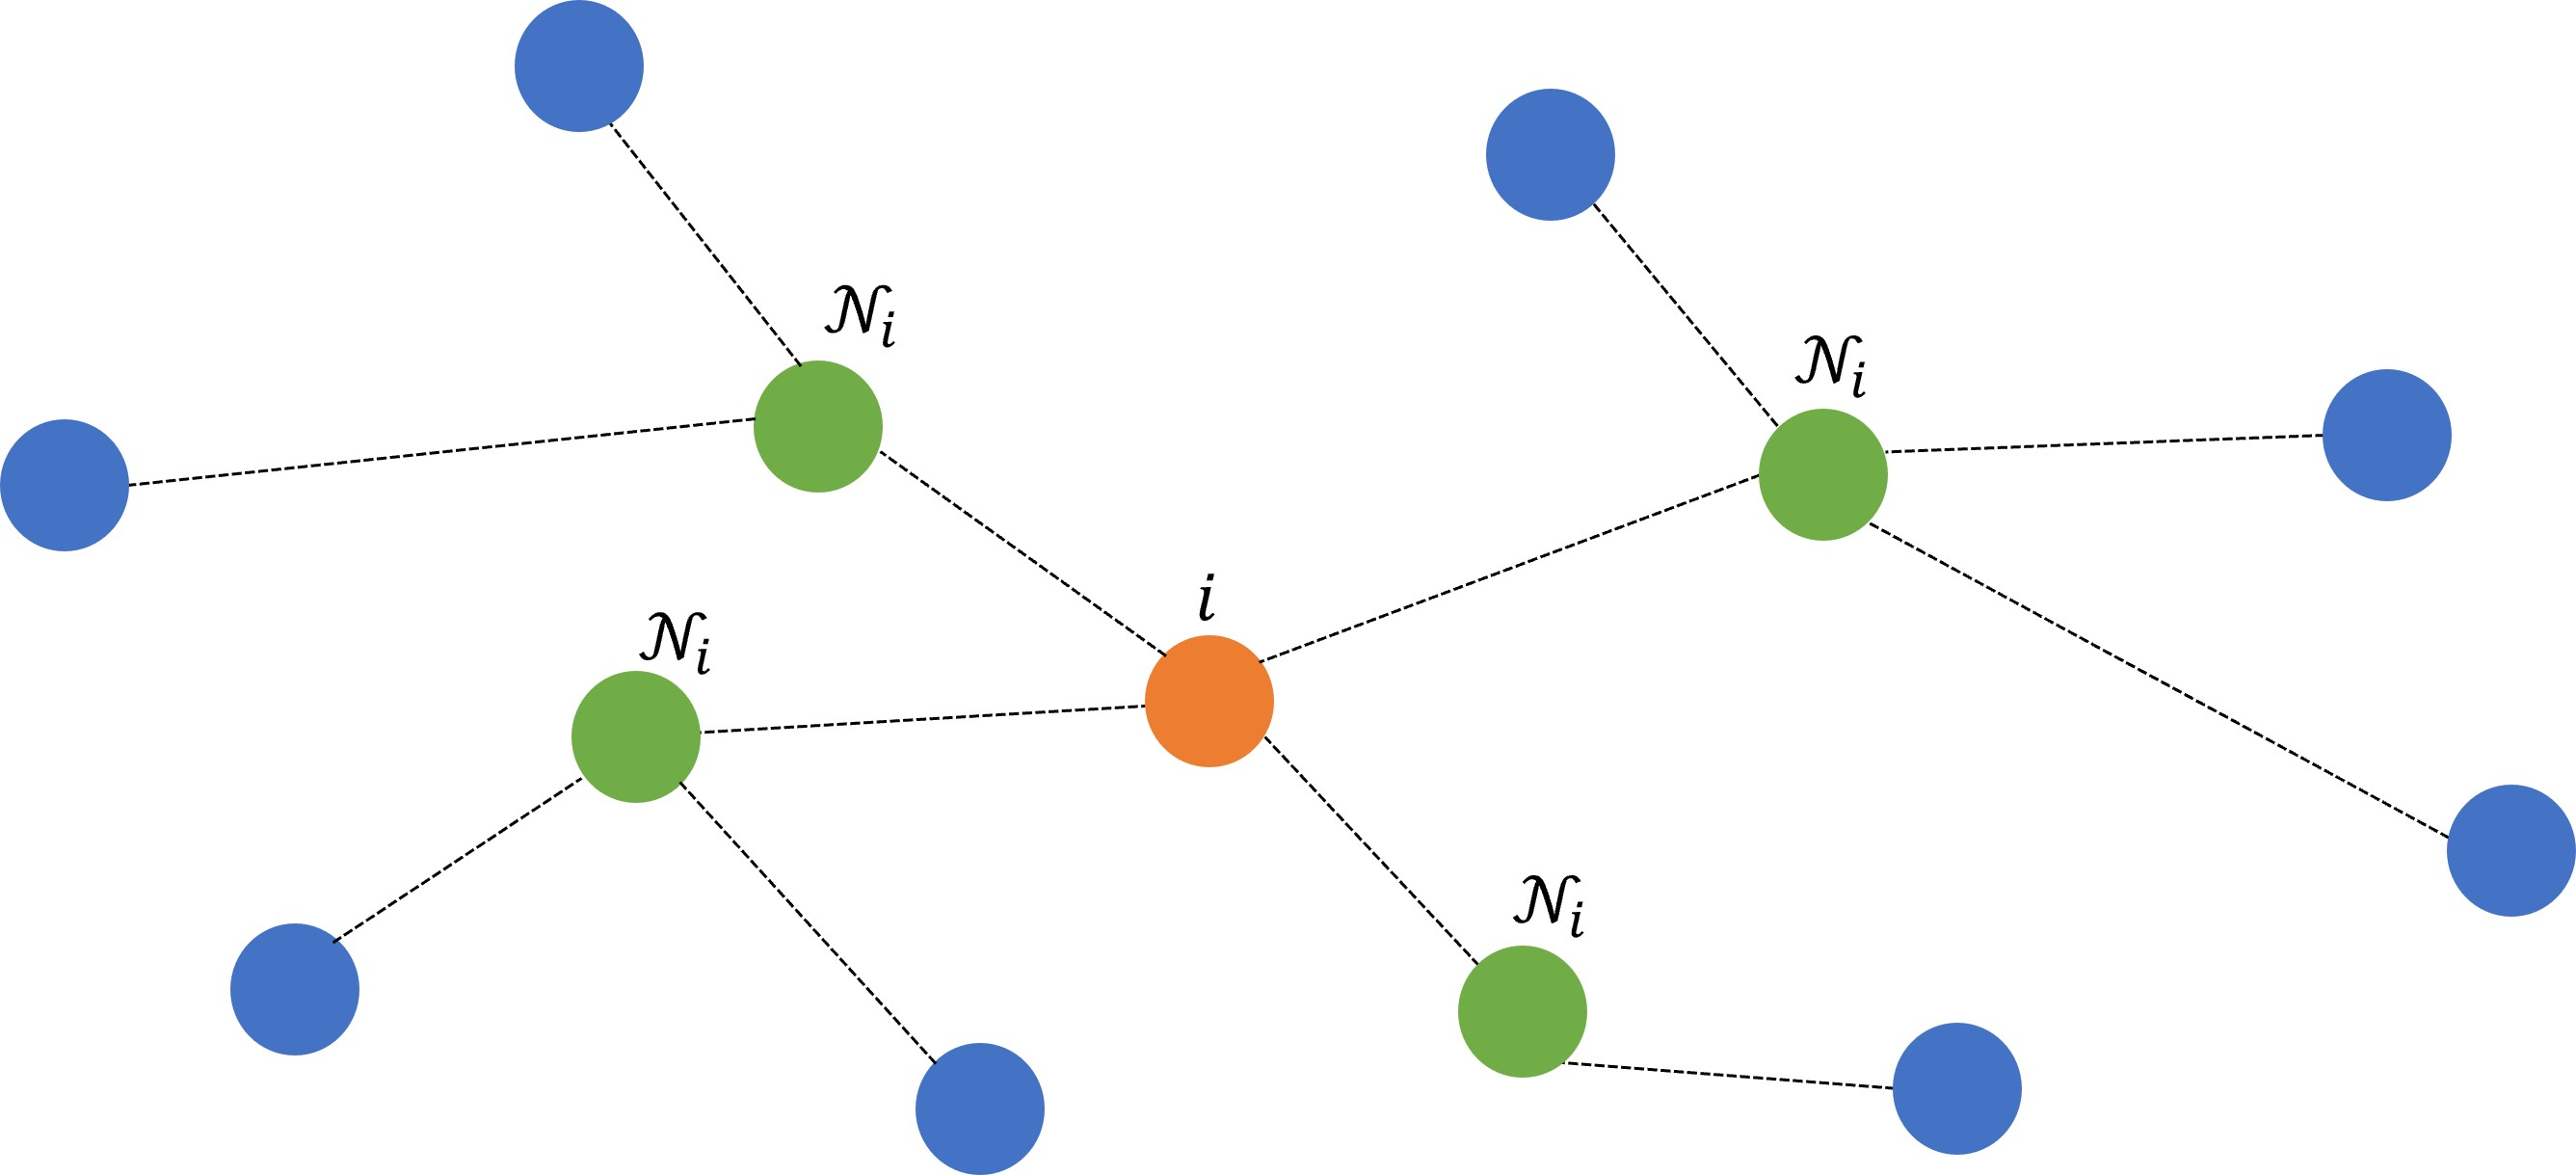
\includegraphics[width=0.7\linewidth]{figures/Graph示意图.jpg}
    \caption{Graph示意图}
    \label{fig:Graph示意图}
\end{figure}

（2）图注意力网络的运算方式

图注意力网络（Graph Attention Networks, GAT）本质上有两种运算方式，掩码图注意力（Mask graph attention）
和全局图注意力（Global graph attention）。掩码图注意力中，图中每个节点$i$只对其邻居节点$\mathcal{N}_{i}$进行注意
力机制的运算；而全局图注意力是图中每个顶点$i$都对图上其余全部顶点进行注意力运算。本文采用的是掩码图注意力
（Mask graph attention）。

（3）图注意力网络的计算

图注意力网络（Graph Attention Networks, GAT）的计算步骤如下：

\begin{itemize}
    \item 步骤1：计算注意力系数
\end{itemize}

对于图中的顶点$i$和其邻居节点$i'$（$i'\in \mathcal{N}_{i}$），逐个计算它们之间的注意力系数$e_{i,i'}$，
该系数衡量节点$i'$的特征对节点$i$的重要性，
计算公式如下式（\ref{节点重要性系数}）所示。
% \begin{equation}\label{节点重要性系数}
%     \\e_{i,i'} = a \left( \left[\mathbf{W}h_{i}\Vert \mathbf{W}h_{i'}\right] \right), i' \in \mathcal{N}_i,
% \end{equation}

\begin{equation}\label{节点重要性系数}
e_{i,i'} = \text{LeakyReLU} \left( \mathbf{a}^T \left[ \mathbf{W}h_i \Vert \mathbf{W}h_{i'} \right] \right), i' \in \mathcal{N}_i,
\end{equation}

首先将节点$i$和节点$i'$的特征向量$h_{i}$和$h_{i'}$分别通过一个共享的线性变换，由可学习的权重矩阵$\mathbf{W}$实现，
顶点的特征进行了增维，这是常见的特征增强（feature augment）方法，得到变换后的特征向量
$\mathbf{W}h_{i}$和$\mathbf{W}h_{i'}$。
接着，将变换后的特征向量拼接（concatenate），式中$\Vert$表示拼接操作，
然后通过一个单层前馈神经网络，由可学习的参数向量$\mathbf{a}$表示，得到一个标量值，
再经过一个激活函数，得到注意力系数$e_{i,i'}$。

\begin{itemize}
    \item 步骤2：注意力系数的归一化
\end{itemize}

为了使注意力系数具有可比性，使用$Softmax$函数对其进行归一化处理。计算公式如下式（\ref{注意力系数的归一化}），
其中$\sigma$表示非线性激活函数。
% \begin{equation}\label{注意力系数的归一化}
%     \\\alpha_{i,i'} = \frac{\exp(\sigma(e_{i,i'}))}{\sum_{k \in \mathcal{N}_i} \exp(\sigma(e_{i,k}))}.
% \end{equation}
\begin{equation}\label{注意力系数的归一化}
\alpha_{i,i'} = \frac{\exp(e_{i,i'})}{\sum_{k \in \mathcal{N}i} \exp(e_{i,k})}
\end{equation}

\begin{itemize}
    \item 步骤3：特征加权求和
\end{itemize}

根据归一化后的注意力系数，对节点$i$的邻居节点的特征进行加权聚合，得到节点$i$更新后的特征表示$h_i'$，
融合了图中局部邻域的结构信息，并动态强调了邻居节点的贡献，
计算公式如下式（\ref{特征加权求和}），式中$\sigma$是激活函数。
\begin{equation}\label{特征加权求和}
    \\h_i' = \sigma \left( \sum_{i' \in \mathcal{N}_i} \alpha_{i,i'} \mathbf{W} h_{i'} \right).
\end{equation}

\begin{itemize}
    \item 步骤4：多头注意力机制
\end{itemize}

可以采用多头注意力机制来增强模型的表达能力，若有$K$个注意力头，对于每个注意力头$k$，重复上述
步骤1 - 3，得到$\{h_i^{'(1)},...,h_i^{'(k)},... h_i^{'(K)}\}$，按需合并。

拼接输出（中间层）：如果不是最终的图注意力层，将$K$个注意力头的输出进行拼接，得到节点$i$的最终
特征表示为下式（\ref{非最终层}）。
\begin{equation}\label{非最终层}
    \\h_i' = \|_{k = 1}^{K} h_i^{'(k)}.
\end{equation}

平均输出（最终层）：如果是最终的图注意力层，将$K$个注意力头的输出进行平均，得到节点$i$的最终特征表示
为下式（\ref{最终层}）。
\begin{equation}\label{最终层}
    \\h_i' = \frac{1}{K} \sum_{k = 1}^{K} h_i^{'(k)}.
\end{equation}

\subsection{构建事件图网络（Event Graph Network）}
参考Wang等人\cite{wang2021reducing}的研究，
本文基于车辆运行的时空轨迹图来构建事件图，用$G(V,E)$表示，其中$V$和$E$分别代表点集和边集，
定义事件图时忽略了公交车站的编号，如下图\ref{fig:事件图}所示。
\begin{figure}[!ht]
    \centering
    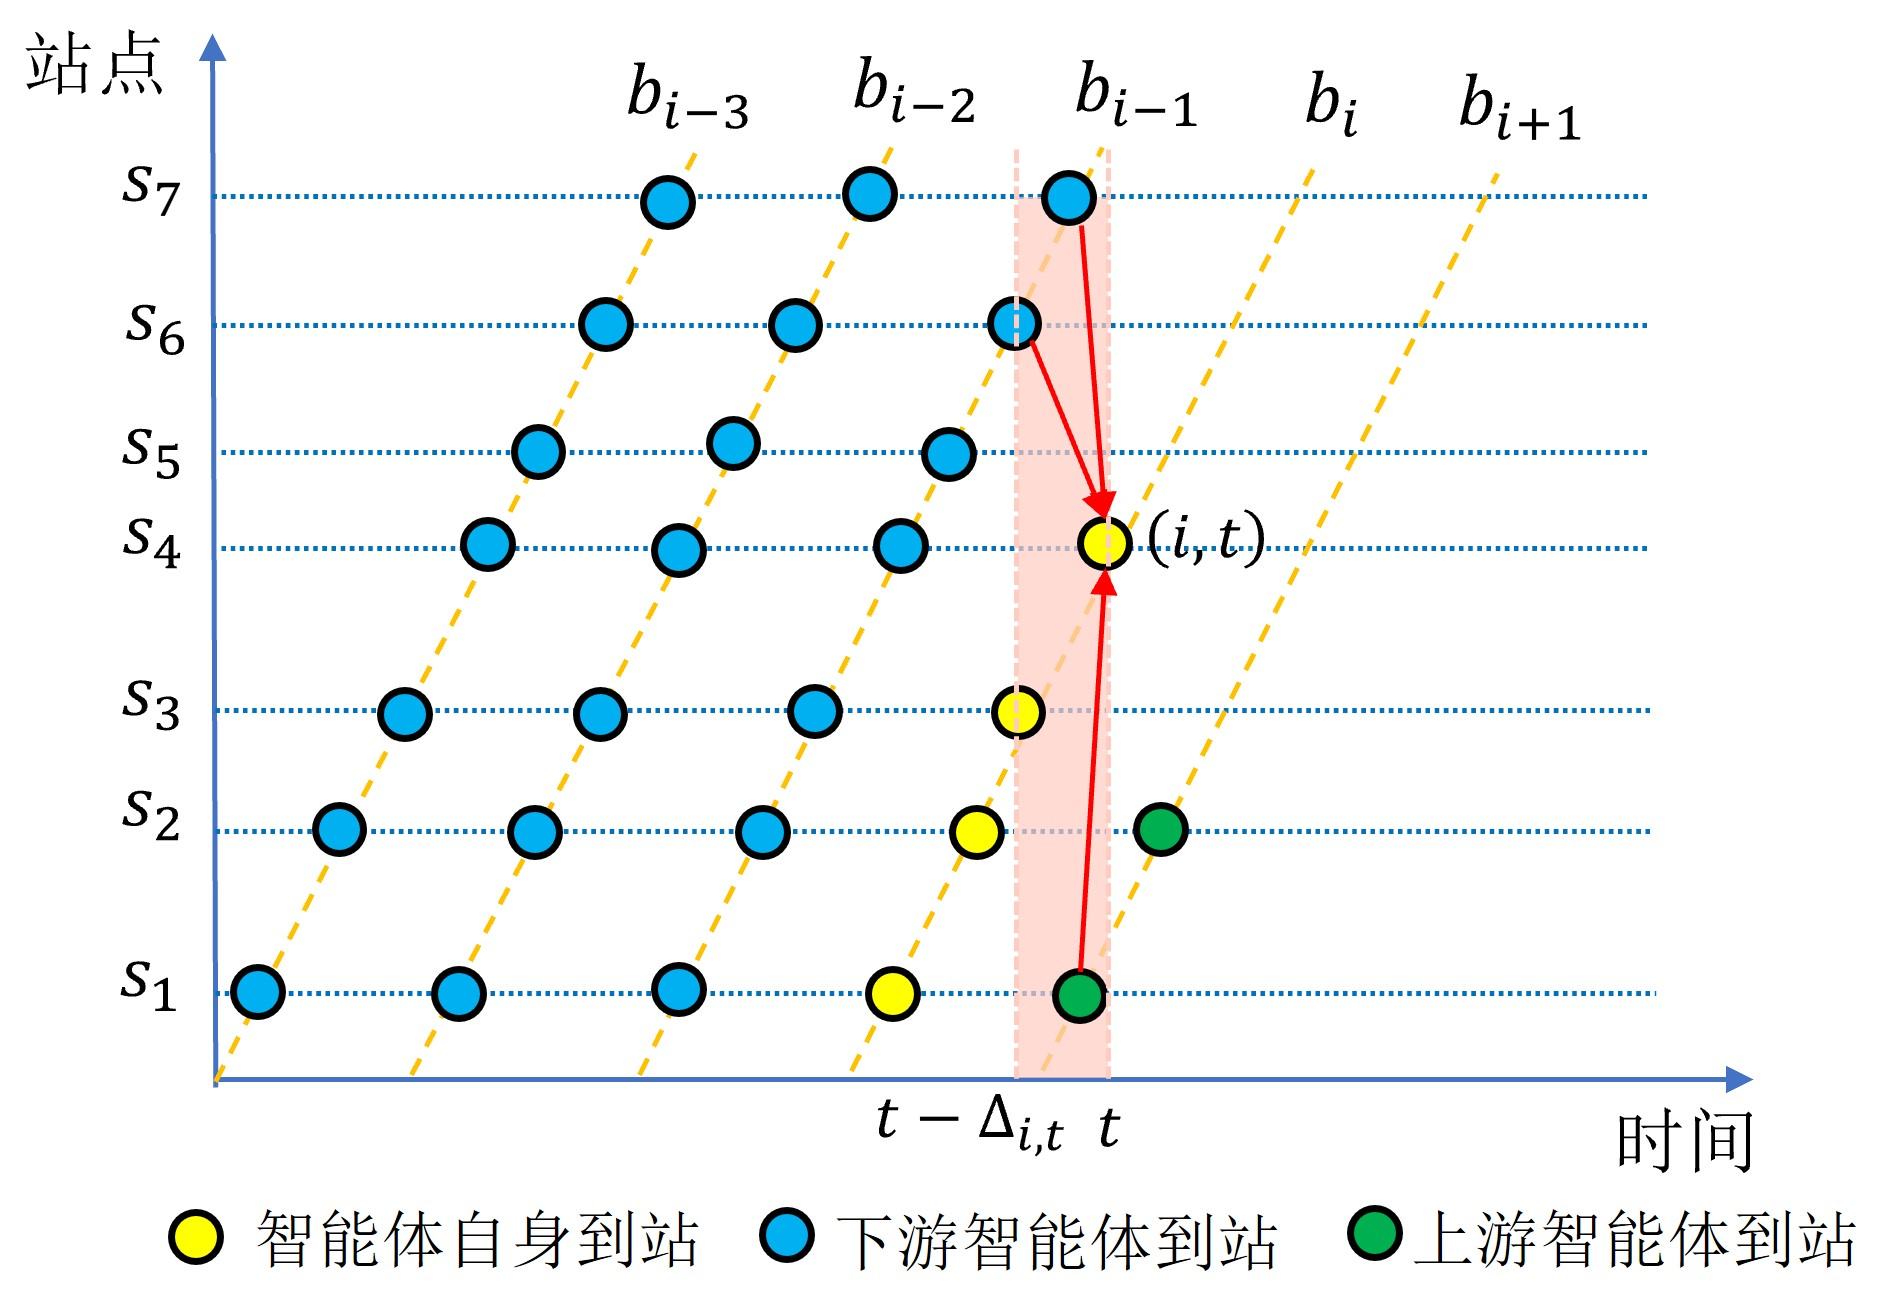
\includegraphics[width=0.7\linewidth]{figures/事件图.jpg}
    \caption{智能体（公交）到站事件图}
    \label{fig:事件图}
\end{figure}

图中的每个节点都表示一个公交车辆到站的事件。
将顶点$(i,t)$定义为公交$b_i$在时刻$t$到达公交车站的事件。
假设公交车辆$b_i$在$t-\triangle_{i,t}$时刻到达一个公交站点，在$t$时刻到达下一个公交站点，
在时间窗$t-\triangle_{i,t} < t' \leq t$内其他车辆（即$b_{i'} \neq b_i$）的所有到达事件$(i',t')$
为节点$(i,t)$的进入边，在本文中，考虑到公交系中车辆的影响通常是局部的，前后两辆车的情况
对公交车辆的驻站决策影响最大，而更远的车辆对当前车辆的影响较小，因此，在$t-\triangle_{i,t} < t' \leq t$
时间窗内的进入边只考虑目标车辆前后两辆车到站情况的影响。
以事件$(i,t)$为例，如上图\ref{fig:事件图}所示，有三条来自其他事件的进入边。
用$\mathcal{N} _{i,t}=\{(i',t') \in V : i'\neq i,t-\triangle_{i,t}<t'\leq t\} $表示
事件$(i,t)$的邻居集合。

对于系统中的每个智能体，事件图可以简明、动态的表征其他智能体的影响，便于进行归纳图学习，
使得在异步控制中智能体可以评估其他智能体的状态、动作对当前智能体决策的影响，使当前智能体
可以更好的学习策略。
具体来说，本文采用图注意力网络（Graph Attention Networks, GAT）来归纳学习和近似其他智能体
动作的影响。考虑到公交上下游车辆对其影响的不同，根据车辆的发车顺序将邻居集合分为上下游事件分别考虑，为上游事件和下游事件分别引入了一个图注意力网络（GAT）。
因此，将$\mathcal{N} _{i,t}$分为两个子集：上游事件集$ \mathcal{N}^u_{i,t} $和下游事件集$ \mathcal{N}^d_{i,t}$，
表达式见下式（\ref{上游事件集}）和（\ref{下游事件集}）。
\begin{equation}\label{上游事件集}
    \\\mathcal{N}^u_{i,t}=\{(i',t') \in V : i'> i,t-\triangle_{i,t}<t'\leq t\},
\end{equation}
\begin{equation}\label{下游事件集}
    \\\mathcal{N}^d_{i,t}=\{(i',t') \in V : i'< i,t-\triangle_{i,t}<t'\leq t\}.
\end{equation}

对于上游事件，节点特征由两部分组成：

一是其他智能体的节点特征$h_{i',t'}=(s_{i',t'},a_{i',t'},e^1_{i',t'},e^2_{i',t'})$，
其中$(s_{i',t'},a_{i',t'})$是智能体$i'$在$t'$时刻的状态动作对；
$e^1_{i',t'}$表示发生两个控制事件的公交车站的间隔，用系统中的总车站数量进行归一化，
$e^2_{i',t'} = |i'- i|$ 是公交车辆$b_{i'}$和$b_i$之间的车辆数量。

二是自身节点特征$h_{i,t}=(s_{i,t},a_{i,t},\text{zeroslike}(e_{i',t'}))$，其中
zeroslike$(e_{i',t'})$表示用零补齐$e_{i',t'}$所占的位数，以确保特征长度相同。
由于事件图是无向的，因此图注意力实际上是基于自身事件与其上游事件之间的关系。
注意力系数可由下式（\ref{上游单个节点注意力系数}）计算，
\begin{equation}\label{上游单个节点注意力系数}
\alpha_{(i,t)(i',t')} = \frac{\exp\left(\text{LeakyReLU}\left(\mathbf{a}^T [\mathbf{W}^a h_{i,t} \| \mathbf{W}^a h_{i',t'}]\right)\right)}{\sum_{(i',t')\in\mathcal{N}_{i,t}^u} \exp\left(\text{LeakyReLU}\left(\mathbf{a}^T [\mathbf{W}^a h_{i,t} \| \mathbf{W}^a h_{i',t'}]\right)\right)},
\end{equation}
% \begin{equation}\label{上游单个节点注意力系数}
%     \\\alpha_{(i,t)(i',t')} = \frac{\exp\left(\sigma\left(f\left(\mathbf{W}^a h_{i,t} \| \mathbf{W}^a h_{i',t'}\right)\right)\right)}{\sum_{(i',t')\in\mathcal{N}_{i,t}^u} \exp\left(\sigma\left(f\left(\mathbf{W}^a h_{i,t} \| \mathbf{W}^a h_{i',t'}\right)\right)\right)},
% \end{equation}
根据得到的注意力权重$\alpha_{(i,t)(i',t')}$,对所有上游邻居节点的变换特征加权求和，得到当前节点的新特征，
如下式（\ref{上游单个特征加权求和}）所示：
\begin{equation}\label{上游单个特征加权求和}
    \\h'_{i,t} = \sum_{(i',t')\in\mathcal{N}^u_{i,t}} \alpha_{(i,t),(i',t')} \mathbf{W}^a h_{i',t'},
\end{equation}
将上游所有节点的特征加权求和，如下式（\ref{上游节点特征加权求和}）所示：
\begin{equation}\label{上游节点特征加权求和}
    \\M^u_{i,t} = \sum_{k\in\{(i,t)\cup\mathcal{N}^u_{i,t}\}} \sigma\left(h_{k}\right),
\end{equation}
下游事件$\mathcal{N}^d_{i,t}$的特征加权聚合$M^d_{i,t}$方式与上游事件相同，
将$M^u_{i,t}$和$M^d_{i,t}$拼接后输入到前馈神经网络，得到加权后的其他智能体的信息向量，见下式（\ref{拼接上下游聚合结果}）。
% 将$M^u_{i,t}$和$M^d_{i,t}$的总和输入到前馈神经网络，得到加权后的其他智能体的信息向量。 
本文没有考虑自注意力机制，且若自身智能体不存在上游事件和下游事件，即没有其他智能体的影响，
会屏蔽输出的聚合值。
\begin{equation}\label{拼接上下游聚合结果}
    \\M_{i,t} = MLP([M^u_{i,t} \|M^d_{i,t}] ).
\end{equation}


\subsection{改进MAPPO强化学习算法}

MAPPO（Multi-Agent Proximal Policy Optimization）是PPO算法在多智能体上的扩展，包含两个网络：
策略网络（参数化表示为$ \pi _{\theta }$）和评价网络（参数化表示为$V_{\phi }$）。
针对多智能体场景下的公交驻站控制问题，本研究提出一种改进的MAPPO算法，其核心创新点体现在策略网络
（Actor）与评价网络（Critic）的结构设计：
\begin{itemize}
    \item 基于图注意力机制的策略网络
\end{itemize}

在原始MAPPO算法的策略网络（Actor）中嵌入
图注意力网络（Graph Attention Networks, GAT）来量化相邻智能体驻站控制动作对当前智能体的影响，
使智能体能自适应关注关键邻居的决策，提升协同控制能力，作出更优控制决策。
\begin{itemize}
    \item 去中心化评价网络
\end{itemize}

评价网络（Critic）进行去中心化设计，采用局部观测建模，仅融合当前智能体自身的观测及相邻智能体的观测，
这样做的原因，一方面是公交系统车辆状态传播具有时空局部性，前后车辆交互占主导；
% 前后两辆车的状态对当前车辆的影响最大，更远的车辆影响较小。
另一方面显著降低模型的计算复杂度，
提升模型的效率，尤其是在大规模车队场景中。
% 这样做在车辆数量较大的公交系统中，可以降低模型的计算复杂度，。

改进MAPPO算法的策略网络和评价网络的结构如下图\ref{fig:策略网络}和图\ref{fig:评价网络}所示。
\begin{figure}[!ht]
    \centering
    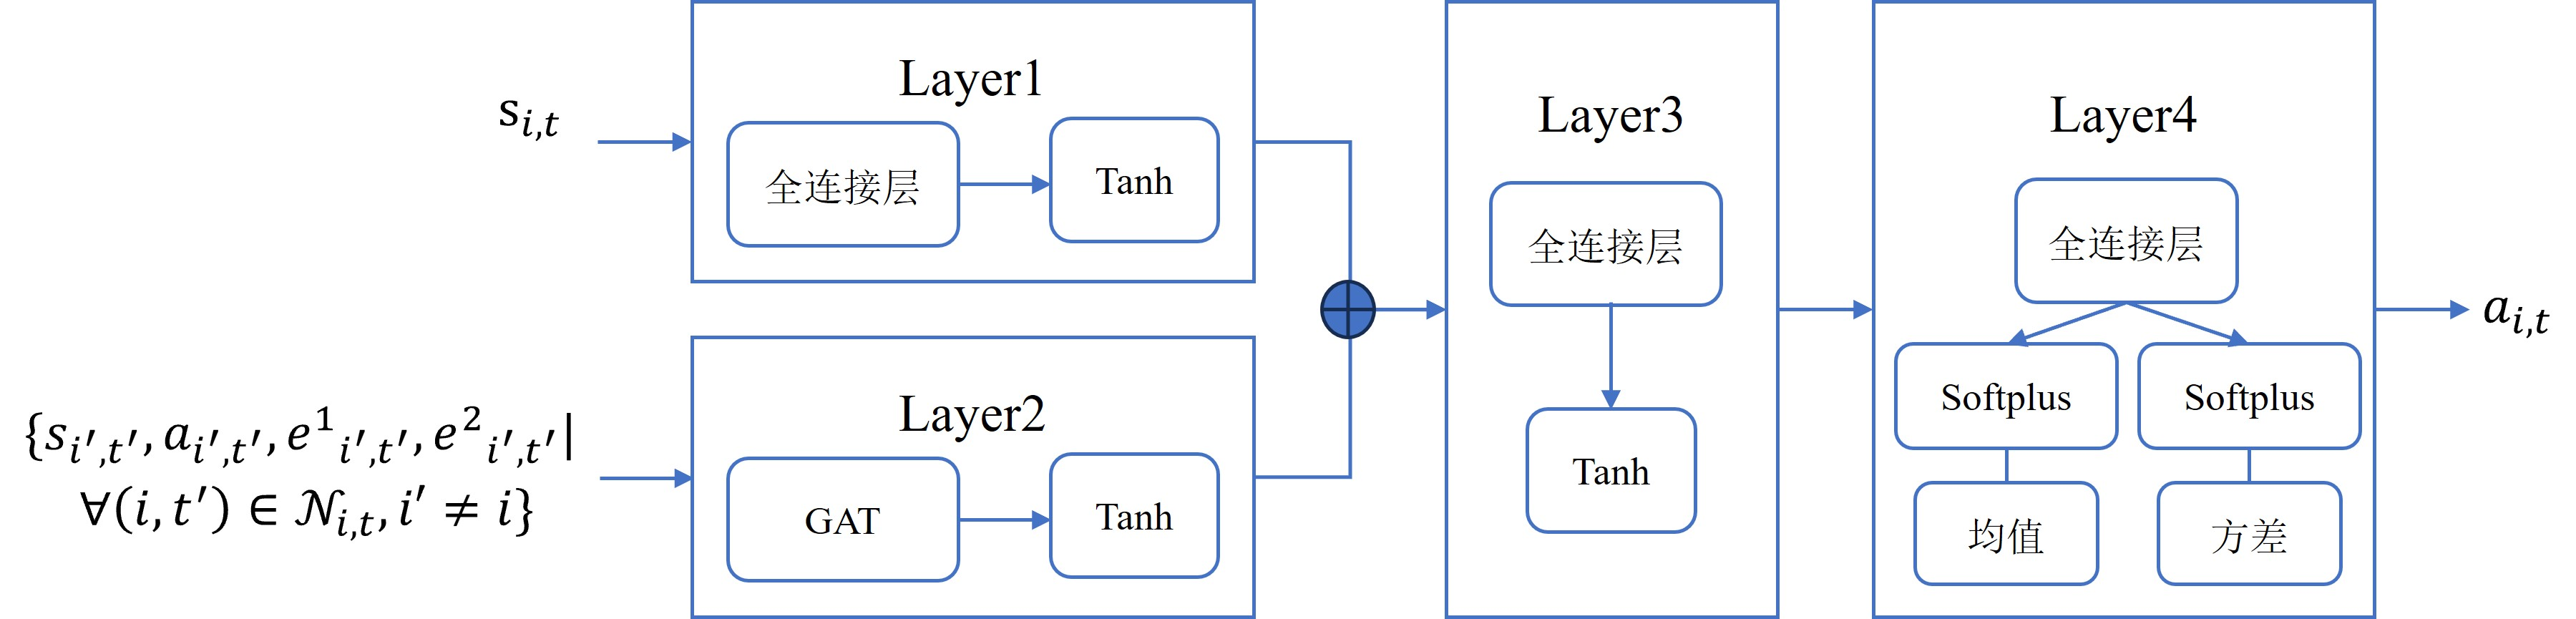
\includegraphics[width=1.\linewidth]{figures/策略网络.jpg}
    \caption{改进MAPPO算法策略网络结构}
    \label{fig:策略网络}
\end{figure}
\begin{figure}[!ht]
    \centering
    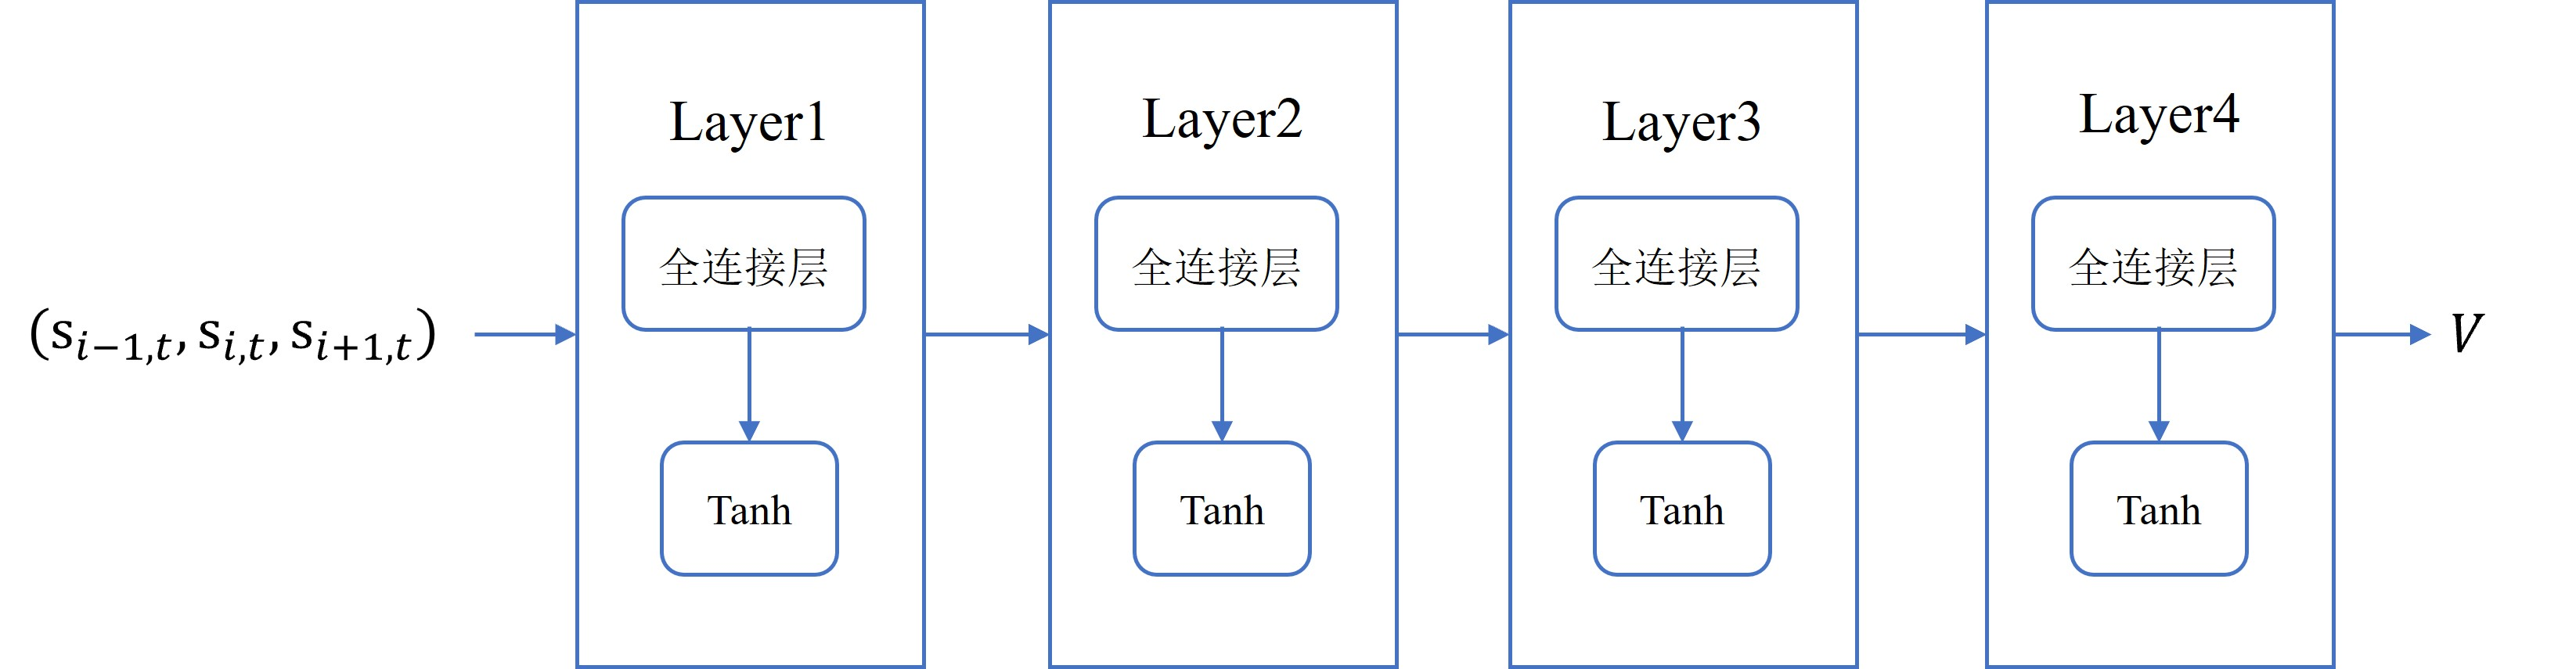
\includegraphics[width=1.\linewidth]{figures/评价网络.jpg}
    \caption{改进MAPPO算法价值网络结构}
    \label{fig:评价网络}
\end{figure}

在本文提出的公交系统中，所有的车辆都是同质的，因此改进MAPPO算法中所有智能体
共用一套网络参数，策略网络$ \pi _{\theta }$的目标是学习一个策略，即
学习一个从观测空间到一个高斯分布的动作均值和方差的映射用于采样动作，使智能体
能够获得尽可能大的累计奖励。评价网络$V_{\phi }$学习一个映射：$\mathcal{S}  \rightarrow R $，
将状态空间$\mathcal{S}$映射到实数$R$，用于估计状态价值。
%\begin{equation}\label{累计折扣奖励}
%   \\J(\theta) = \mathbb{E}_{a_{i,t},s_{i,t}}\left[\sum_t \gamma^t R\left(s_{i,t}, a_{i,t}\right)\right]
%\end{equation}

策略网络的优化目标为：
\begin{equation}\label{策略网络的优化目标}
\begin{split}
    L(\theta) &= \left[\frac{1}{Bn} \sum_{k = 1}^{B} \sum_{i = 1}^{n} \min \{ r_{\theta,k}^{(i)} A_{k}^{GAE(\gamma,\lambda )(i)}, \text{clip}\left(r_{\theta,k}^{(i)}, 1 - \epsilon, 1 + \epsilon\right) A_{k}^{GAE(\gamma,\lambda )(i)}\} \right] \\
    &+ \sigma \frac{1}{Bn} \sum_{k = 1}^{B} \sum_{i = 1}^{n} S\left[\pi_{\theta}\left(s_{k}^{(i)},M^{(i)}_{k}\right)\right],
\end{split}
\end{equation}
其中，$r_{\theta,k}^{(i)}$表示表示新旧策略之比，见下式（\ref{比率}），
$A_{k}^{GAE(\gamma,\lambda )(i)}$是优势函数，采用广义优势估计（Generalized Advantage Estimation，GAE）方法估计，
见下式（\ref{优势函数}），用于衡量一个动作相对于平均水平的好坏，$\lambda$ 是GAE特有的参数，权衡偏差和方差的超参数；
$S$表示策略的熵，$\gamma$是折扣因子，$\sigma$为控制熵系数的一个超参数。
\begin{equation}\label{比率}
    \\r_{\theta,k}^{(i)} = \frac{\pi_{\theta}\left(a_{k}^{(i)}|s_{k}^{(i)},M^{(i)}_{k}\right)}{\pi_{\theta_{\text{old}}}\left(a_{k}^{(i)}|s_{k}^{(i)},M^{(i)}_{k}\right)},
\end{equation}
\begin{equation}\label{优势函数}
    \\A_{k}^{GAE(\gamma,\lambda )(i)} = \sum_{l = 0}^{\infty} (\gamma\lambda )^l \cdot (r_k + \gamma V^{k + l + 1}_{\phi_{\text{old}}} - V^{k + l}_{\phi_{\text{old}}}).
\end{equation}

评价网络的优化目标为：
\begin{equation}\label{评价网络的优化目标}
\begin{split}
    L(\phi) &= \frac{1}{Bn'} \sum_{k = 1}^{B} \sum_{i = 1}^{n'} \left( \max \left\{  \left(V_{\phi} \left(s_{k}^{(i)}\right) - \hat{R}^{GAE(\gamma,\tau)}_{k}\right)^2, \right.\right. \\
    &\left.\left. \left( \text{clip}\left(V_{\phi} \left(s_{k}^{(i)}\right), V_{\phi_{\text{old}}} \left(s_{k}^{(i)}\right) - \varepsilon, V_{\phi_{\text{old}}} \left(s_{k}^{(i)}\right) + \varepsilon\right) - \hat{R}^{GAE(\gamma,\tau )}_{k}\right)^2 \right\}  \right),
\end{split}
\end{equation}
式中，$\hat{R}^{GAE(\gamma,\lambda)}_{k}$是累计折扣奖励，见式(\ref{折扣奖励})，$B$表示批次的大小，$n'$表示包含自身和相邻智能体的数量。
\begin{equation}\label{折扣奖励}
    \\\hat{R}^{GAE(\gamma,\lambda)}_{k} = A_{k}^{GAE(\gamma,\lambda)(i)}+ V_{\phi_{old}} \left(s_{k}^{(i)}\right).
\end{equation}

改进MAPPO算法伪代码如下表\ref{tab3-2}所示。
% \usepackage{longtable} % 引入 longtable 宏包
\begin{table}[!ht]
\centering
\caption{改进的MAPPO算法流程}
\resizebox{\textwidth}{!}{
\label{tab3-2}
\begin{tabular}{p{0.9\textwidth}}
\toprule
\textbf{改进的MAPPO算法伪代码}\\
\midrule
初始化Actor网络$\pi$的参数$\theta$以及Critic网络$V$的参数$\phi$，
设置每次模拟的时间范围为$T$个时间步，
设置学习率$\alpha$，
设置经验回放池$D=\{M_1=[],M_2=[],...,M_n=[]\}$\\
1.for $episode = 1,2,...,E$：\\
2.\hspace{1em}for $t = 1,2,...T$:\\
3.\hspace{1em}\hspace{1em}for 公交车辆$b_i =1 ,2,...,n$： \\
4.\hspace{1em}\hspace{1em}\hspace{1em}if 公交车辆$b_i$到达站点$s_j$并且不是第一次到达站点：\\
5.\hspace{1em}\hspace{1em}\hspace{1em}\hspace{1em}获取当前状态$s_{i,t}$以及本次到站与上一次到站时间间隔内相邻车\\
\hspace{1em}\hspace{1em}\hspace{1em}辆的到站信息$\mathcal{N} _{i,t}$\\
6.\hspace{1em}\hspace{1em}\hspace{1em}\hspace{1em}基于$\pi_{\theta_{old}}(a_{i,t}|(s_{i,t},M_{i,t}))$
采样得到动作$a_{i,t}$\\
7.\hspace{1em}\hspace{1em}\hspace{1em}\hspace{1em}执行动作并获得奖励$r_{i,t}$
和下一个状态$s_{i,t''}$\\
8.\hspace{1em}\hspace{1em}\hspace{1em}\hspace{1em}将$(s_{i,t},a_{i,t},r_{i,t},s_{i,t''},\mathcal{N} _{i,t})$
存储到经验回放池的\\
9.\hspace{1em}\hspace{1em}end for\\
10.\hspace{1em}end for \\
11.\hspace{1em}for 公交车辆$b_i =1 ,2,...,n$：\\
12.\hspace{1em}\hspace{1em}使用广义优势估计(GAE)计算优势估计值$\widehat{A}$，见式(\ref{优势函数}) \\
13.\hspace{1em}\hspace{1em}基于$V_{\phi}(s_{i-1,t},s_{i,t},s_{i+1,t})$计算计算状态价值 \\
14.\hspace{1em}\hspace{1em}使用式(\ref{折扣奖励})计算累计回报$\widehat{R} $并进行归一化处理 \\
15.\hspace{1em}for $k = 1,2,...,K$：\\
16.\hspace{1em}\hspace{1em}从经验回放池$D$中选取包含所有智能体数据的小批量数据$b$ \\
17.\hspace{1em}\hspace{1em}使用式(\ref{策略网络的优化目标})更新$\theta$ \\
18.\hspace{1em}\hspace{1em}使用式(\ref{评价网络的优化目标})更新$\phi$ \\
19.\hspace{1em}end for \\
20.end for\\
\bottomrule
\end{tabular}
}
\end{table}



\section{基于强化学习驻站控制的公交运行流程}

\subsection{公交运行控制流程}

在完成基于改进MAPPO算法的公交驻站控制模型的建立后，为验证模型性能，本研究构建了完整的模型仿真
运行流程，如下图\Ref{fig:基于强化学习的公交运行流程}所示，具体实现过程如下：

\begin{figure}[!ht]
    \centering
    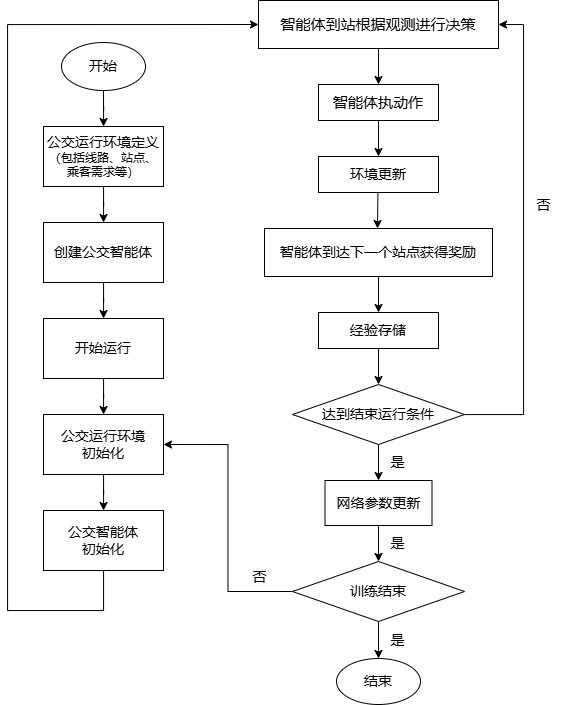
\includegraphics[width=0.8\linewidth]{figures/公交运行仿真设计.png}
    \caption{基于强化学习驻站控制的公交运行流程}
    \label{fig:基于强化学习的公交运行流程}
\end{figure}

（1）公交运行环境构建

囊括公交运行所涉及的各类关键要素。具体涵盖站间距离的精准设定、站点位置布局，
以及乘客需求的模拟生成等，通过对这些要素的系统性整合与精确构建，
真实还原公交实际运行场景。


（2）公交智能体的创建

确定智能体数量，创建与之对应的同质智能体集合。
对智能体进行参数化设定，涵盖公交车辆动力学参数，如公交运行速度、额定载客量等关键指标。
同时，完成智能体动作空间与观测空间等的配置设置，明确智能体可执行动作的范围以及可感知环境信息的维度。


（3）系统初始化和训练控制

首先进行环境初始化，设置环境参数并重置状态，其次完成智能体初始化。此外还需要
初始化算法参数，包括策略网络与价值网络及超参数。每轮训练前都要完整重复系统初始化，
确保各轮训练环境一致。
训练控制环节，合理设置训练循环，确定
训练总轮数、每轮最大步数及终止条件，借助经验回放池进行数据存储与处理。


（4）在线决策和经验积累

当智能体到达站点时，会立即获取实时环境状态信息，随后将观测到的状态信息输入策略网络，策略
网络基于输入的状态信息生成动作概率分布，智能体依据概率分布选择具体动作，并执行该动作。
在智能体与环境交互过程中，产生的相关信息会被组成含状态、动作、奖励等要素的
经验元组，存入经验回放池，打破数据时间相关性，随着训练过程的推进，经验回放池中的经验元组不断积累，
为网络更新提供数据，有助于算法更高效地学习到最优策略。


（5）模型训练和性能验证

训练时从经验回放池里采样数据，先计算优势函数，据此构建经裁剪处理的目标函数，
进而计算策略网络梯度，用优化器更新参数；
同时，依据采样数据计算目标价值，通过均方误差损失函数计算价值网络预测值与目标价值的误差，
更新价值网络参数。
选取评价指标用测试集数据观察智能体依当前策略网络的表现，判断性能是否达标。
经多次验证分析模型稳定性，若不达标则调整超参数或改进模型结构，重新训练与验证。


\subsection{公交运行控制场景的Python实现}

（1）Python环境要求

依赖库：numpy>=1.19.2、matplotlib>=3.3.3、torch>=1.7.0、pandas>=1.2.0

（2）主要文件和模块

\begin{itemize}
    \item 主程序文件：负责初始化公交系统和模拟引擎，并启动模拟循环。
\end{itemize}

\begin{itemize}
    \item 模型文件夹：包含强化学习模型的实现： MAPPO 算法和改进 MAPPO 算法。
\end{itemize}

\begin{itemize}
    \item 模拟文件夹：公交系统模拟的核心代码，包含公交、公交站、乘客、模拟引
\end{itemize}
擎等，类的定义和功能见下表\ref{tab3-11}所示。

\begin{itemize}
    \item 结果文件夹：用于存储模拟结果。
\end{itemize}

\begin{table}[!ht]
\centering
\caption{公交控制仿真环境中类的定义及功能}
\label{tab3-11}
\begin{tabular}{>{\centering\arraybackslash}m{3.5cm} >{\raggedright\arraybackslash}m{9.6cm} }
\toprule
\textbf{类} & \textbf{功能} \\
\midrule
Bus 类 & 表示公交车，包含公交车的基本属性（如 ID、线路 ID、发车时间、在车乘客等）和操作方法（如移动、停靠、上下客等）\\
BusStop 类  & 表示公交站点，包含站点的基本属性（如 ID、位置等）和乘客生成方法。  \\
Passenger 类 & 表示乘客，包含乘客的基本属性（如 ID 、起始站点、到站时间、上下车用时等）\\
SimulationEngine 类 & 模拟引擎，负责公交系统的整体模拟和控制，包括强化学习控制逻辑\\
\bottomrule
\end{tabular}
\end{table}

（3）主要流程
\begin{itemize}
    \item 初始化：在主程序文件中调用模拟文件夹中模拟引擎类的初始化方法，读
\end{itemize}
取公交站点和线路信息，初始化公交车列表、线路列表和初始化模拟时间步。
\begin{itemize}
    \item 模拟运行：在模拟引擎类中，通过调用模拟方法模拟运行，主要步骤如下：\\
    （a）公交车调度：根据调度时间，判断是否有公交车需要发车；\\
（b）公交车移动：每个时间步更新每辆公交车的位置，判断是否到达站点；\\
（c）乘客上下车：如果公交车到达站点，调用模拟引擎类中的服务方法处理乘客的上下车操作，
具体的，首先调用公交类中的乘客下车方法，让需要下车的乘客下车，并更新相关信息，如在车乘客列表、
乘客下车总用时等；接着调用站点生成乘客的方法，生成新的乘客，并让符合条件的乘客上车。 \\
（d）强化学习控制：调用强化学习控制方法，根据当前状态选择动作，对公交车进行驻站控制；\\
（e）更新状态和奖励：更新公交车、站点和乘客的状态，并计算奖励。
\end{itemize}

（4）强化学习控制

\begin{itemize}
    \item 观测状态：通过公交类的属性获取其相邻车辆的总行程，从而根据运行速
\end{itemize}
度得到前后向车头时距；根据当前公交车和站点信息从存储数据中获得在车乘客数量。

\begin{itemize}
    \item 选择动作：调用智能体选择动作的方法将观测状态作为输入得到动作。
\end{itemize}

\begin{itemize}
    \item 计算奖励：根据公交车和乘客的状态变化，计算奖励信号。
\end{itemize}

（5）模拟结束

当模拟达到指定的时间步或满足其他结束条件时，模拟结束。此时可以调用模拟引擎中的
数据统计方法计算统计信息，如乘客等待时间、车辆驻站时间等。



% \section{案例分析}
% \subsection{实验设置}
% 本文中的实验使用PyCharm搭建模拟环境，算法训练过程使用Python 3.9和PytTorch 2.0.0实现。

% 本文实验的公交系统，设计为一条单向环形公交线路，环形线路上由$m=$ 12个公交站点，公交站点均匀分，
% 公交车队由$n=$ 6辆同质公交车组成，如上图\ref{fig:公交线路与站点示意图}所示。
% 系统中公交车辆均以$v=$ 20 km/h的速度匀速运行，
% 在相邻两个站点的站间运行时间为3 min（不包括站点乘客的上下车用时和公交的驻站时间），
% 因此两个相邻的公交站点之间的距离为1 km。
% 每个公交车辆都从起始站点$s_1$发出按顺序发车，沿着线路运行，车辆发车时间间隔$H=$ 360 s，
% 所有车辆在到达的第一个站点（即发车站点）不进行驻站控制。
% 公交车辆的容量限制$U=$ 80个乘客。乘客上下车的时间参考Chen L\cite{chen2016real}等人的设置，
% 每位乘客的上车时间$t_b=$ 3 s，下车时间$t_a=$ 1.8 s。设置车辆在站点的最大驻站时间$\triangle T =$180 s，
% 当车辆在站点的驻站时间小于30 s时忽略不计，视为车辆不驻站。

% 在环形线路公交系统运行开始后，公交从发车站点沿着环形线路不断运行，
% 直到达到系统设定的停止时间步即结束运行。

% 每个公交站点乘客到达遵循泊松过程，各个公交站点乘客的到达率如下图\ref{fig:乘客到达率}所示。
% 乘客的下车站点在其上车站点后的$\lfloor$ m / 2 $\rfloor $站点中随机选择。每个公交站点
% 积累乘客的时间为相邻车辆到达站点的时间间隔，当公交站点第一次有公交到站时，其累积乘客的时间
% 为4 min。
% \begin{figure}[!ht]
%     \centering
%     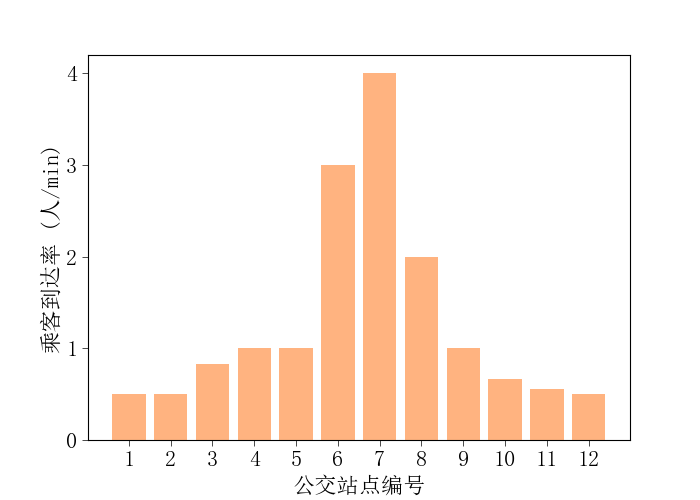
\includegraphics[width=0.65\linewidth]{figures/环形线路公交站点乘客到达率.png}
%     \caption{公个公交站点乘客到达率}
%     \label{fig:乘客到达率}
% \end{figure}

% \subsection{评价指标}
% 基于乘客和公交运行商的角度评价公交服务的效率和可靠性，因此，本文选择了如下四个评价指标：

% （1）平均驻站时间（AHT）

% 平均驻站时间是在模拟运行期间公交车辆在每个站点的平均驻站时间，该指标反映了驻站控制策略对
% 公交运行的干预程度，同时也反映了在车乘客由于公交驻站增加的额外行程时间。

% （2）平均等待时间（AWT）

% 平均等待时间是在模拟运行期间系统中每位乘客在站点的平均等待时间，该指标可以很好的量化
% 公交的服务水平和可靠性。

% （3）平均旅行时间（ATT）

% 平均旅行时间是在模拟期间，所有乘客从到达站点等待上车到完成整个行程下车离开站点，整个过程中的平均用时，
% 该指标能够表征公交的运行效率和服务水平。

% （4）平均占用离散度（AOD）

% 平均占用离散度是每个站点所有公交车辆占用率的离散程度的均值，车辆占用率的离散度用车上乘客数量的方差和均值之比表示，
% 该指标可以用来评价公交服务的可靠性和乘客的出行乘坐体验，因为当公交车发生串车时，
% 前车通常会挤满乘客，而后车几乎是空的，公交车辆的载客量出现高度不均的现象，AOD值会很大。
% 用车上乘客数量的方差和均值的比值来计算，
% 表达式见下式（\ref{平均占用离散度}）。
% \begin{equation}\label{平均占用离散度}
%     Var(o_{i,j}) / E(o_{i,j})
% \end{equation}

% \subsection{对比模型}

% 将通过改进的MAPPO算法训练得到多智能体驻站控制策略（MH）与以下的基准模型进行比较，其中包含基于
% 规则的控制模型（基于固定车头时距、时刻表的控制模型）、传统的数学优化模型（基于
% 前向车头时距、后向车头时距的控制模型）和基于原始的MAPPO强化学习算法的驻站控制模型。

% （1）无控制模型（NH）

% 无控制模型中，不进行任何干预，但由于本文提出的公交系统不允许超车，
% 所以当发生串车时，后面的车辆将被强制驻站。

% （2）基于固定车头时距的控制模型（HH）

% 基于固定车头时距的控制模型是进行简单的控制，驻站控制在实际车头时距小于
% 计划车头时距时触发，驻站时间$th=H_0-h^-$，
% $H_0$是计划车头时距，本文参考Chen W\cite{chen2016real}等人的研究，将$H_0$设置为6 min。

% （3）基于时刻表的控制模型（SH）

% 基于时刻表驻站的控制模型中，公交车辆的到站时间小于时刻表给定的时间就会触发驻站控制。
% 在这种情况下，若公交的到站时间大于给定时刻表设定的到站时间，公交在该站点不需要进行
% 驻站控制，若公交早于给定时刻表的到达站点，要驻站到给定的发车时间时才能离开站点。

% （4）基于前向车头时距的控制模型（FH）

% Daganzo\cite{daganzo2009headway}2009年提出了基于前向车头时距的控制模型是，
% 驻站时间由下式（\ref{基于前向车头时距的驻站控制}）决定，
% \begin{equation}\label{基于前向车头时距的驻站控制}
%     th = max\{ 0,\overline{d}+g(H_0 - h^-) \} 
% \end{equation}
% 其中，$H_0$是计划车头时距,$\overline{d} $是平衡时的平均延误，$g>$0是一个控制参数。
% 我们使用与Daganzo\cite{daganzo2009headway}相同的参数。

% （5）基于后向车头时距的控制模型（BH）

% 基于后向车头时距的控制模型是Xuan\cite{xuan2011dynamic}等人2011年提出的优化模型，
% 驻站时间$th= \beta h^+$，$ h^+$是到达公交站的后向车头时距，$\beta$
% 是要设置的参数，取值为0.5。

% （6）基于MAPPO算法训练的控制模型（MAPPO）

% 将改进的模型与传统的MAPPO算法模型
% 的训练结果进行比较，传统的MAPPO算法模型没有引入图注意力网络，
% 将不考虑智能体到站的异步特性的影响，为了比较所提出的改进模型的优势，
% 两个模型使用的算法参数保持相同。

% \subsection{模型训练}
% 对提出强化学习模型进行了300个回合的训练，每个回合进行3 h模拟，其中预热时间为25 min。
% 强化学习算法超参数的取值如下表\ref{tab3-3}所示。
% \begin{table}[!ht]
% \centering
% \caption{改进的MAPPO算法超参数的取值}
% \label{tab3-3}
% \begin{tabular}{cccp{0.1\textwidth}}
% \toprule
% \textbf{参数} & \textbf{取值} &  \textbf{参数} & \textbf{取值}\\
% \midrule
% 策略网络$Actor$的学习率 & 1e-4  &  $Adam$优化器$eps$参数 & 1e-5\\
% 价值网络$Critic$的学习率 & 1e-4  & 折扣因子$\gamma $ & 0.9\\
% 策略网络$Actor$的梯度裁剪阈值 & 4 & $GAE$的参数$\lambda $ & 0.95 \\
% 价值网络$Critic$的梯度裁剪阈值 & 5 & 裁剪参数$ \epsilon $ & 0.2\\
% 策略熵的系数$\beta $ & 0.01  & 小批量大小B &  64\\
% 每个小批量的更新次数 &  3 & 注意力头数$K$ & 2 \\
% 激活函数负斜率 & 0.2  \\
% \bottomrule
% \end{tabular}
% \end{table}

% 模型训练结果见下图\ref{fig:改进的多智能体强化学习模型的训练结果}所示，
% 图中分别展示了策略网络和评价网络的训练结果。
% 在策略网络的训练结果图中，
% 蓝色线条表示每个训练回合智能体获得的累积奖励，橙色线条表示为
% 15个训练回合的滑动平均值。
% 从图中可以看出，算法的收敛速度较快，累积奖励曲线在较早阶段就可以取得明显优化效果，
% 由于强化学习算法的探索性和公交系统存在的随机性，累积奖励存在波动。
% \captionsetup{justification=centering} % 设置题注内容居中
% \begin{figure}[!ht] 
%     \centering
%     \begin{subfigure}[t]{0.45\textwidth}
%         \centering
%         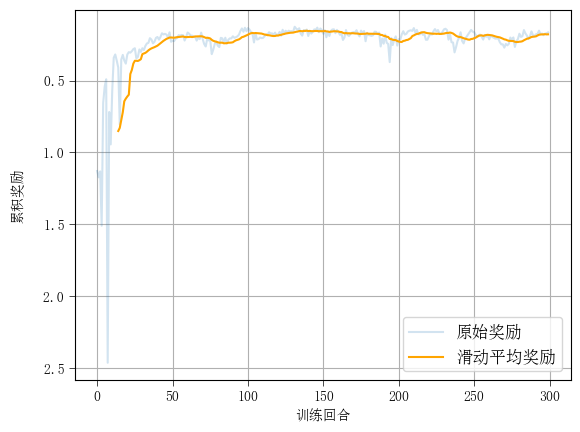
\includegraphics[width=\linewidth]{figures/改进的mappo累积奖励.png}
%         \caption{策略网络每个训练回合的累积奖励}
%     \end{subfigure}
%     \quad
%     \begin{subfigure}[t]{0.45\textwidth}
%         \centering
%         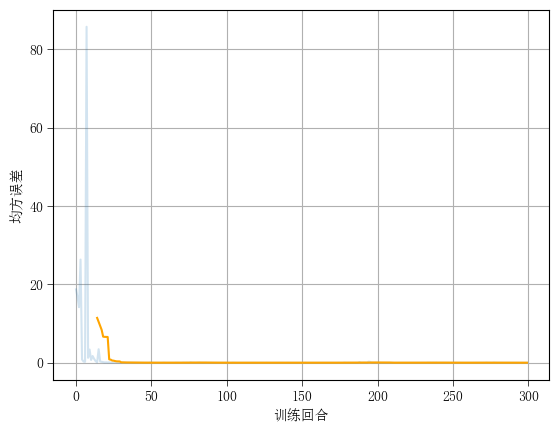
\includegraphics[width=\linewidth]{figures/改进的mappo的均方误差.png}
%         \caption{评价网络的均方误差}
%     \end{subfigure}
%     \caption{改进的MAPPO模型的训练结果}
%     \label{fig:改进的多智能体强化学习模型的训练结果}
% \end{figure}
% \subsection{实验结果与分析}
% 模型训练结束后，对该模型进行测试验证。每个对比模型通过20回合的模拟来评估其可靠性。
% 首先从微观层面进行分析，下图\ref{fig:无控制的车辆运行轨迹}是无控制模型（NH）的公交车辆运行轨迹图，即在系统中不对公交车辆
% 进行任何驻站控制干预。从图中可以看出，在不采取任何干预措施的情况下，系统中的公交车辆
% 很容易发生串车。
% \begin{figure}[!ht]
%     \centering
%     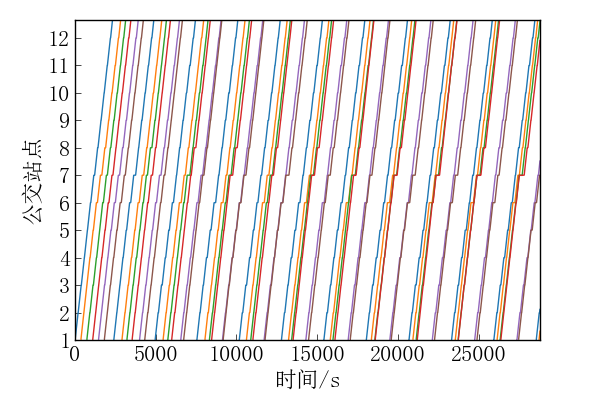
\includegraphics[width=0.5\linewidth]{figures/NH车辆轨迹.png}
%     \caption{无控制的车辆运行轨迹}
%     \label{fig:无控制的车辆运行轨迹}
% \end{figure}
% \captionsetup{justification=centering} 
% \begin{figure}[!ht] 
%     \centering
%     \begin{subfigure}[b]{0.47\textwidth}
%         \centering
%         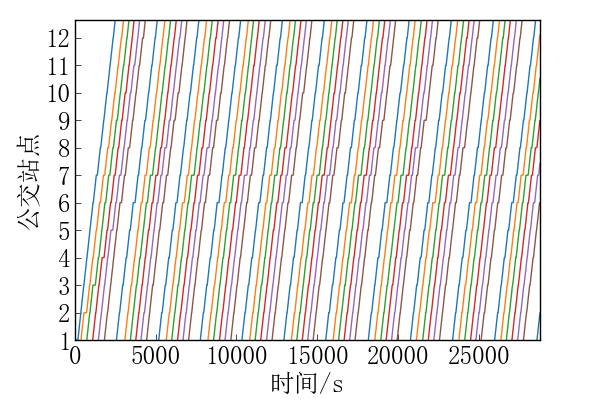
\includegraphics[width=\linewidth]{figures/HH车辆轨迹.png}
%         \caption{基于固定车头时距的控制策略}
%     \end{subfigure}
%     \quad
%     \begin{subfigure}[b]{0.46\textwidth}
%         \centering
%         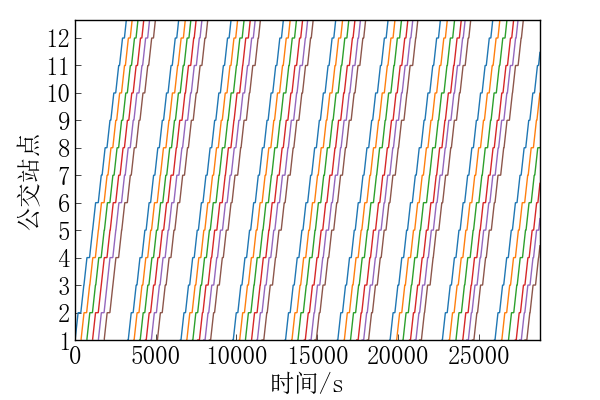
\includegraphics[width=\linewidth]{figures/SH车辆轨迹.png}
%         \caption{基于时刻表的控制策略}
%     \end{subfigure}
%     \vskip 10pt % 子图组间垂直间距
%     \begin{subfigure}[b]{0.46\textwidth}
%         \centering
%         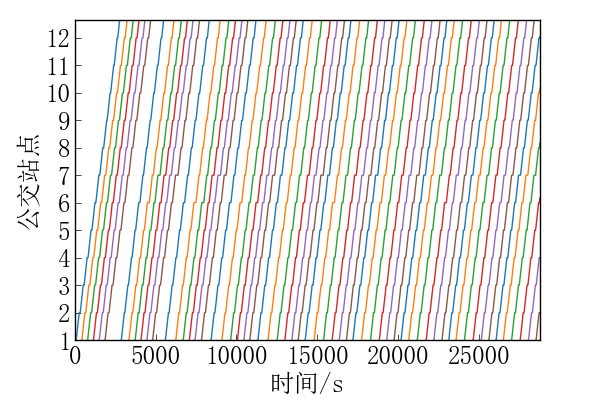
\includegraphics[width=\linewidth]{figures/FH车辆轨迹.png}
%         \caption{基于前向车头时距的控制策略}
%     \end{subfigure}
%     \quad
%     \begin{subfigure}[b]{0.46\textwidth}
%         \centering
%         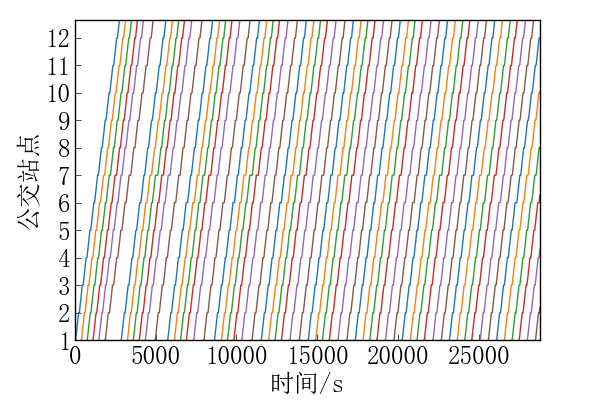
\includegraphics[width=\linewidth]{figures/BH车辆轨迹.png}
%         \caption{基于后向车头时距的控制策略}
%     \end{subfigure}
%     \vskip 10pt % 子图组间垂直间距
%     \begin{subfigure}[b]{0.46\textwidth}
%         \centering
%         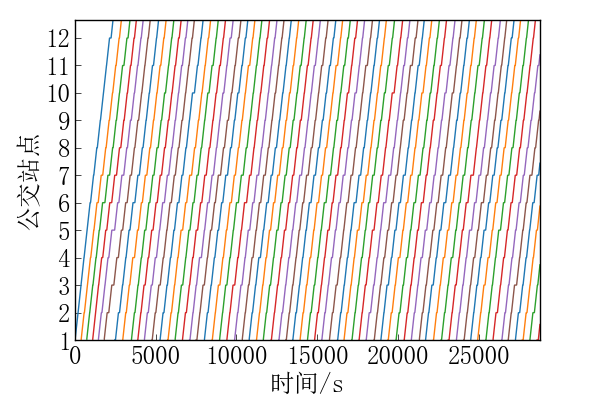
\includegraphics[width=\linewidth]{figures/MAPPO车辆轨迹.png}
%         \caption{基于MAPPO算法的控制策略}
%     \end{subfigure}
%     \quad
%     \begin{subfigure}[b]{0.46\textwidth}
%         \centering
%         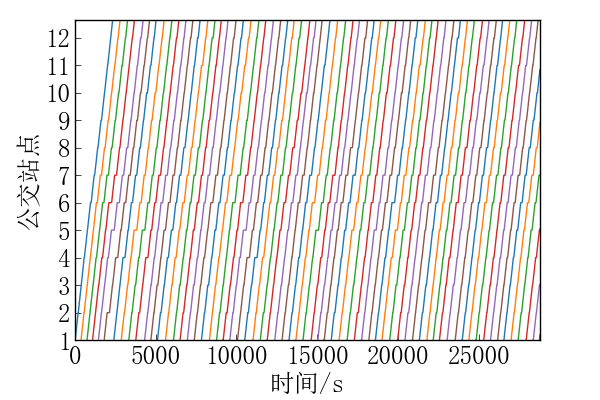
\includegraphics[width=\linewidth]{figures/改进的MAPPO车辆轨迹.png}
%         \caption{基于改进的MAPPO算法的控制策略}
%     \end{subfigure}
%     \caption{不同控制策略下的公交运行车辆轨迹}
%     \label{fig:不同控制策略下的公交运行车辆轨迹}
% \end{figure}

% 下图\ref{fig:不同控制策略下的公交运行车辆轨迹}是本文所提出的
% 基于强化学习的控制模型和其他基准模型的车辆轨迹，
% 基于固定车头时距的控制模型（HH）
% 和基于时刻表的控制模型（SH）视为是基于规则的控制，基于固定车头时距的驻站控制
% 模型（HH）和基于时刻表的控制模型（SH）在一定程度上都可以缓解公交串车的发生，
% 但是基于规则的控制模型对于公交车头时距的不规律问题改善不明显，
% 两种基于规则的控制方法无法灵活有效的处理公交系统存在的不确定性，无法有效实现车头时距的规律性。

% 相比于基于规则的控制，基于前向车头时距的控制模型（FH）、基于后向车头时距的控制模型
% （BH）以及基于强化学习的控制模型（基于MAPPO算法和基于改进的MAPPO算法）的控制策略更具灵活性，
% 从图中的车辆轨迹可以看出，这些策略对于缓解公交串车现象更有效。
% 相比之下，基于强化学习的控制策略表现更优，
% 主要原因是基于强化学习的控制策略中，智能体可以获取更多的实时信息，
% 如智能体的观测状态中包含了乘客信息等，使得智能体的决策更优，减少不必要的干预，
% 而其他控制策略则不能充分利用这一信息，
% 同时基于强化学习的策略还可以考虑决策的长期影响，在改善公交的车头时距偏差的方面
% 表现更佳。

% 下图\ref{fig:不同策略下不同公交站点各车辆的载客量}是整个模拟过程中，
% 不同的控制策略下，系统中公交车辆在每个站点的载客数量，
% 每个子图中的不同线条表示不同的车辆。从图中可以看出，在没有任何控制的情况下，
% 系统中车辆的载客辆高度不均，存在资源浪费，
% 同时从乘客的角度来看，存在部分车辆过度拥挤导致乘客出行体验不佳。
% 基于固定车头时距的控制策略（HH）和基于时刻表的控制策略（SH）对于车辆载客量的均衡
% 改善较小，相比之下，
% 基于前向车头时距的控制策略（FH）和基于前向车头时距的控制策略（BH）有了一定程度的改善，
% 因为他们可以较好的缓解公交串车的发生。
% 同样的，基于强化学习的控制策略表现更优，对比两种强化学习方法，
% 从图\ref{fig:不同策略下不同公交站点各车辆的载客量}(f)和(e)可以看出，
% 本文所提出的基于改进的MAPPO算法的控制策略在均衡车
% 辆载客量方面表现最佳，更有效缓解的了公交传车和载客量不均衡的问题。
% \captionsetup{justification=centering}
% \begin{figure}[htbp]  
%     \centering
%     \begin{subfigure}[b]{0.44\textwidth}
%         \centering
%         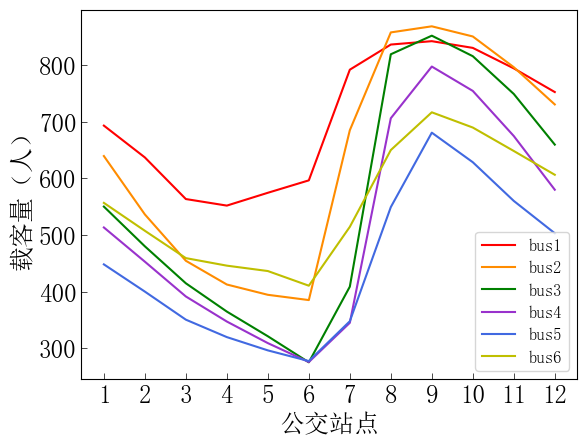
\includegraphics[width=\linewidth]{figures/NH载客量.png}
%         \caption{NH策略的公交载客量}
%     \end{subfigure}
%     \quad
%     \begin{subfigure}[b]{0.44\textwidth}
%         \centering
%         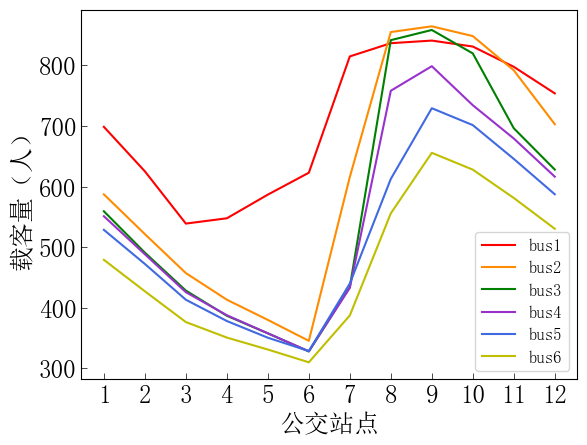
\includegraphics[width=\linewidth]{figures/HH载客量.png}
%         \caption{HH策略的公交载客量}
%     \end{subfigure}
%     \vskip 10pt % 子图组间垂直间距
%     \begin{subfigure}[b]{0.44\textwidth}
%         \centering
%         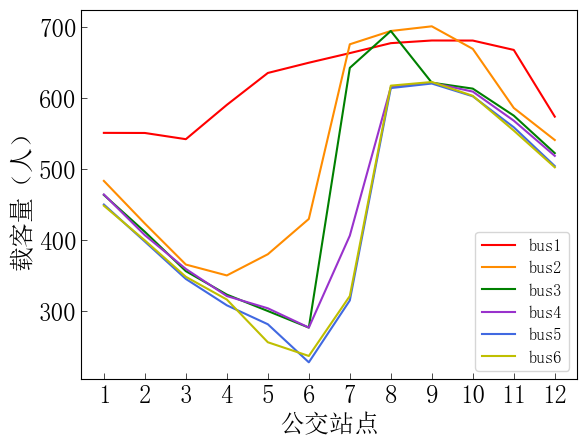
\includegraphics[width=\linewidth]{figures/SH载客量.png}
%         \caption{SH策略的公交载客量}
%     \end{subfigure}
%     \quad
%     \begin{subfigure}[b]{0.44\textwidth}
%         \centering
%         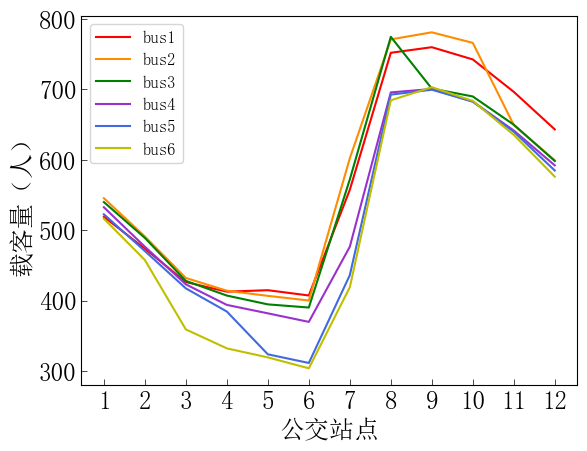
\includegraphics[width=\linewidth]{figures/FH载客量.png}
%         \caption{FH策略的公交载客量}
%     \end{subfigure}
%     \vskip 10pt % 子图组间垂直间距
%     \begin{subfigure}[b]{0.44\textwidth}
%         \centering
%         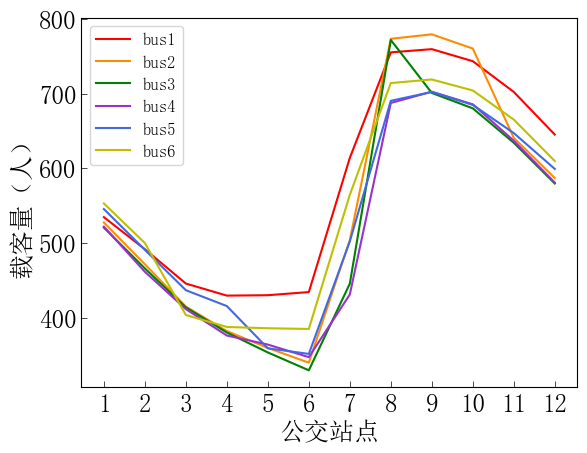
\includegraphics[width=\linewidth]{figures/BH载客量.png}
%         \caption{BH策略的公交载客量}
%     \end{subfigure}
%     \quad
%     \begin{subfigure}[b]{0.44\textwidth}
%         \centering
%         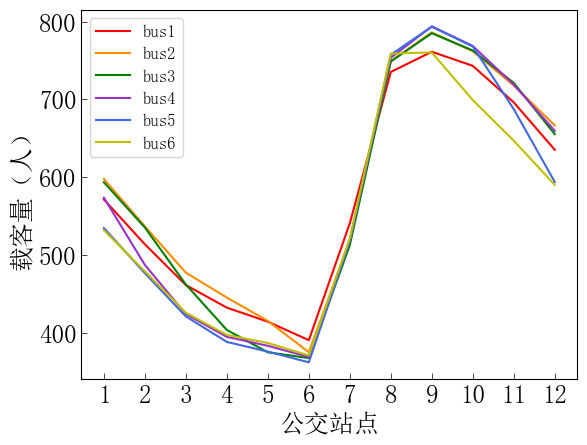
\includegraphics[width=\linewidth]{figures/MAPPO载客量.png}
%         \caption{基于MAPPO算法策略的公交载客量}
%     \end{subfigure}
%     \vskip 10pt % 子图组间垂直间距
%     \begin{subfigure}[t]{0.44\textwidth}
%         \centering
%         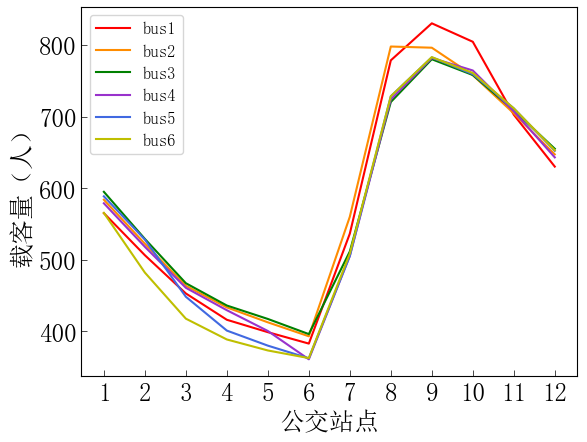
\includegraphics[width=\linewidth]{figures/改进的MAPPO载客量.png}
%         \caption{基于改进的MAPPO算法策略的公交载客量}
%     \end{subfigure}
%     \caption{不同策略下不同公交站点各车辆的载客量}
%     \label{fig:不同策略下不同公交站点各车辆的载客量}
% \end{figure}

% \captionsetup{justification=centering} % 设置题注内容居中
% \begin{figure}[!ht]
%     \begin{minipage}[t]{0.5\linewidth}
%         \centering
%         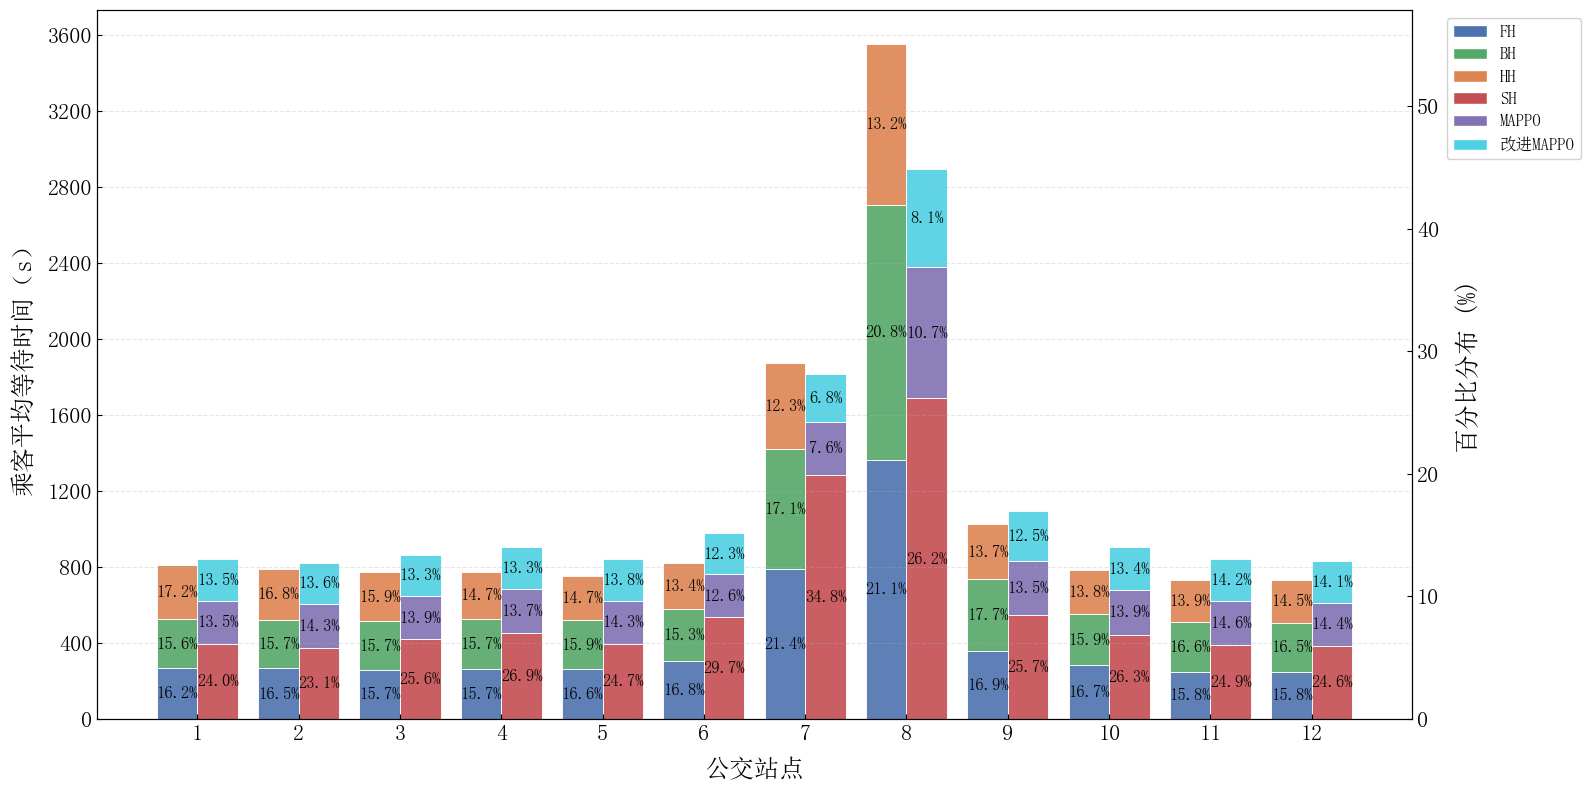
\includegraphics[width=\textwidth]{figures/AWT.png}
%         \caption{不同策略下的乘客平均等待时间\\（AWT）}
%         \label{fig:平均等待时间}
%     \end{minipage}%
%     \begin{minipage}[t]{0.5\linewidth}
%         \centering
%         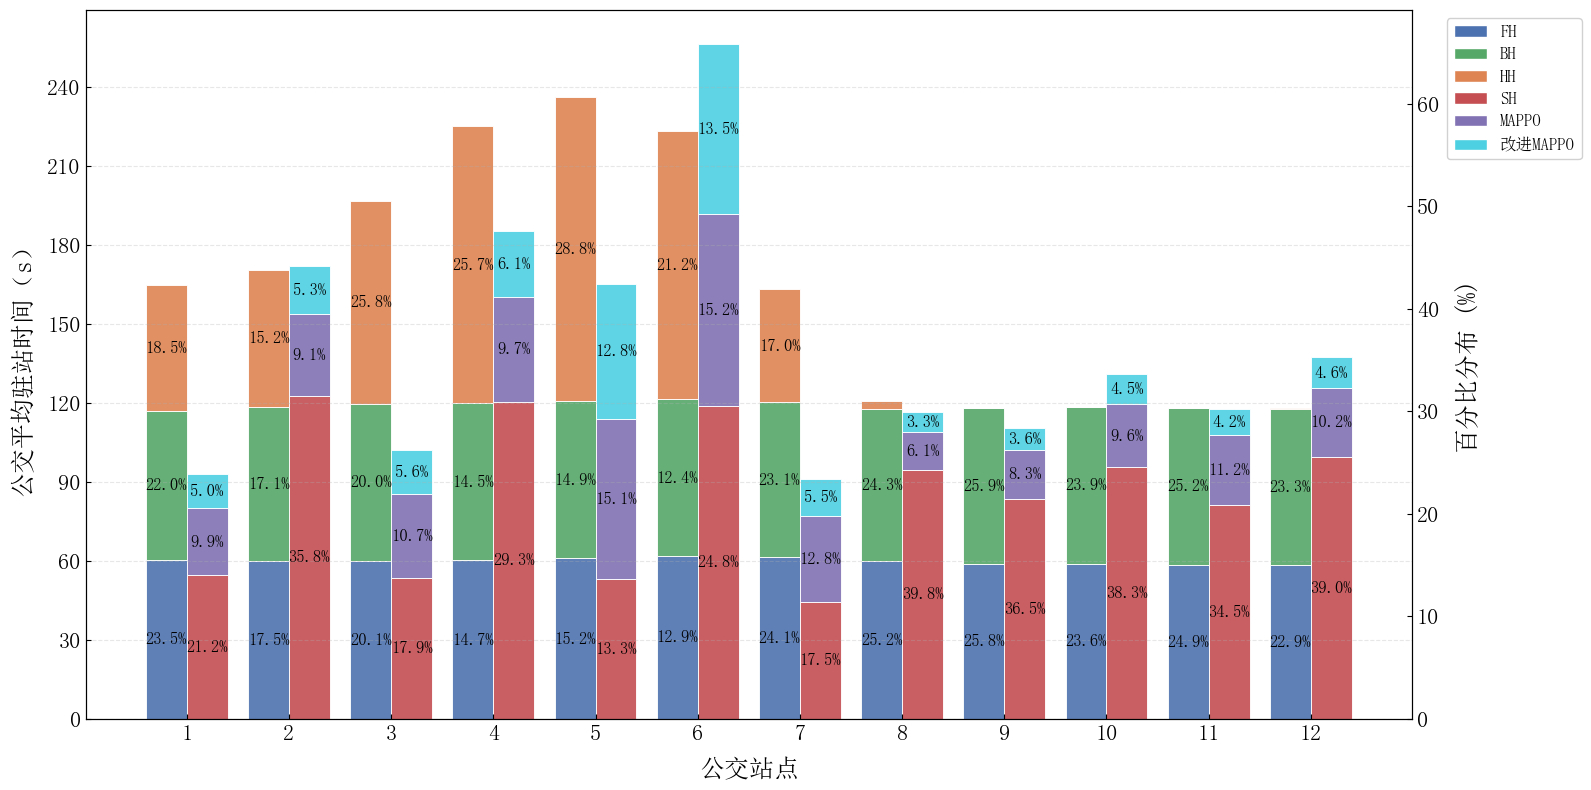
\includegraphics[width=\textwidth]{figures/AHT.png}
%         \caption{不同策略下的车辆平均驻站时间\\（AHT）}
%         \label{fig:平均驻站时间}
%     \end{minipage}
% \end{figure}

% \captionsetup{justification=centering} % 设置题注内容居中
% \begin{figure}[htbp]
%     \begin{minipage}[t]{0.5\linewidth}
%         \centering
%         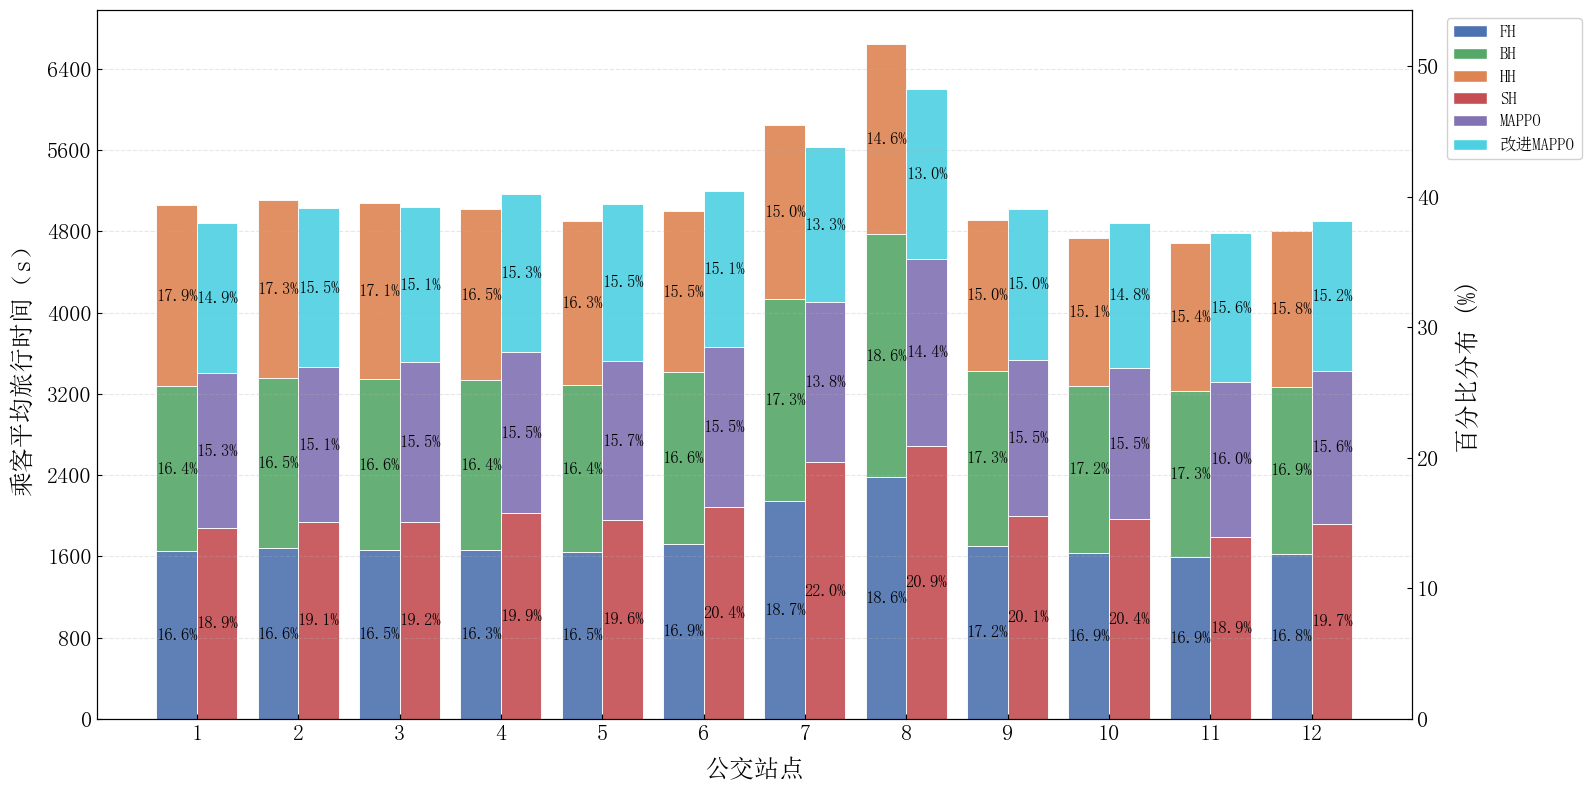
\includegraphics[width=\textwidth]{figures/ATT.png}
%         \caption{不同策略下的乘客平均旅行时间\\（ATT）}
%         \label{fig:平均旅行时间}
%     \end{minipage}%
%     \begin{minipage}[t]{0.5\linewidth}
%         \centering
%         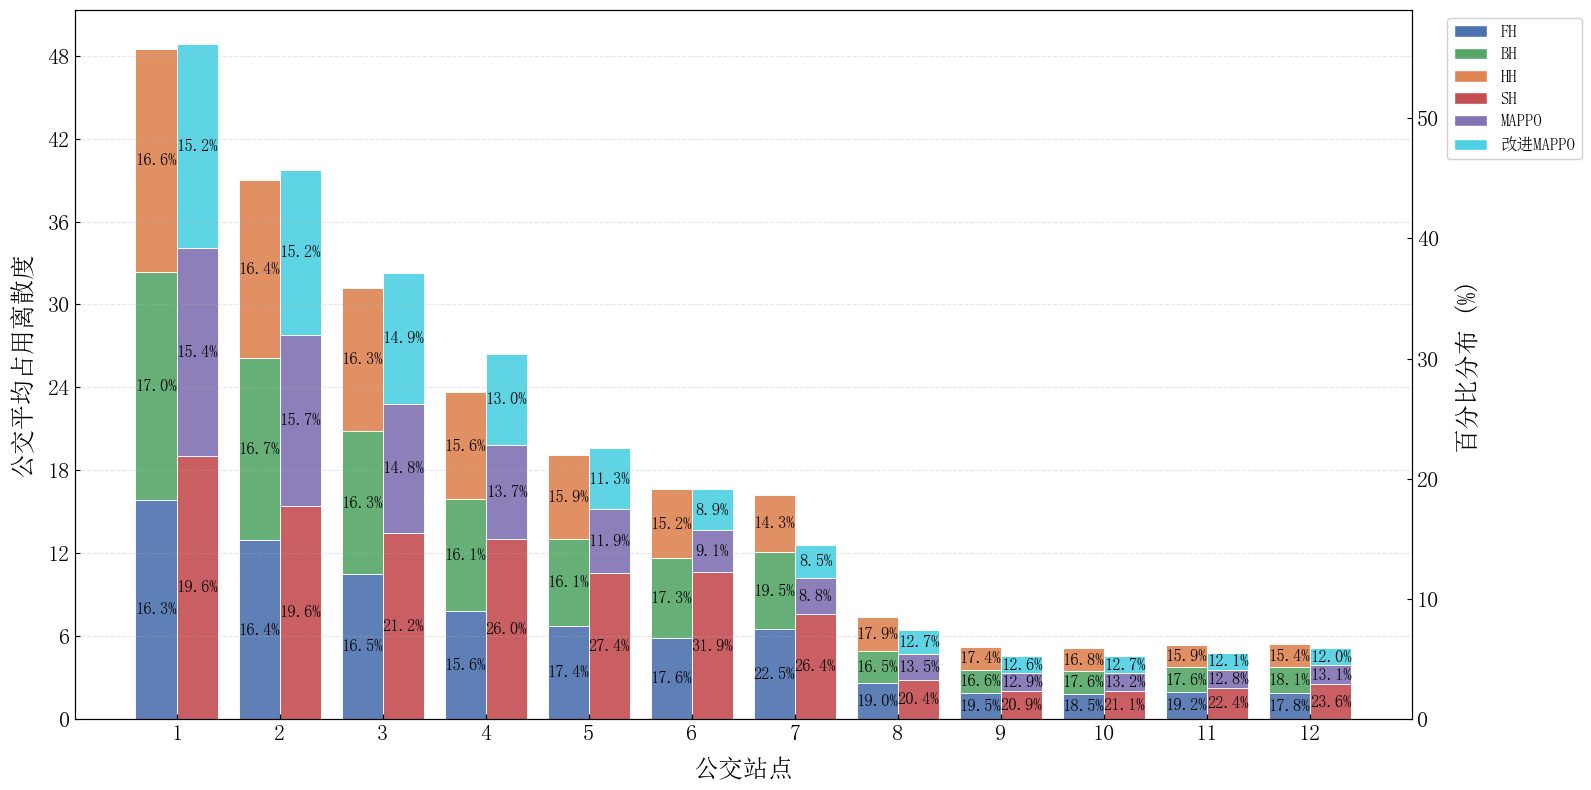
\includegraphics[width=\textwidth]{figures/AOD.png}
%         \caption{不同策略下的车辆平均占用离散度\\（AOD）}
%         \label{fig:平均车辆占用离散度}
%     \end{minipage}
% \end{figure}
% 接下来，从公交系统的宏观层面来进一步分析，图\ref{fig:平均等待时间}是整个公交运行系统中，
% 不同控制策略下在每个公交站点乘客到站等待的平均等待时间（AWT），图中的不同颜色条代表不同控制策略下
% 该指标的值，可以看出，相比于基于优化模型的控制策略（FH和HH），基于强化学的策略（MAPPO和改进的MAPPO）
% 表现更优，在个别站点，基于固定车头时距的控制策略（HH）的平均等待时间是最低的，这可能是由于
% 在该策略下的固定车头时距限制了各站点的最大驻站时间。
% 两种基于强化学习的控制模型，在该指标上的表现差异较小，
% 但提出的改进MAPPO算法的控制策略仍然有更好的表现。

% 图\ref{fig:平均驻站时间}是整个公交系统运行过程中，每个站点车辆的
% 平均驻站时间（AHT），从图中可以看出，仍然是基于强化学习算法的策略在该指标上表现更好，尤其是
% 基于改进的MAPPO算法的驻站控制策略，有更小的驻站时间，这也表明了本文提出的模型可以在
% 施加更小的控制干预下，保持公交系统车头时距的均衡，减少串车的发生。
% 图中基于固定车头时距的控制策略（HH），在$s_{9}$到$s_{12}$站点没有控制干预，而在前面的站点施加了较多
% 的控制干预，原因可能是，在车辆发出的前期通过控制干预保持了车头时距的稳定，所以在后面的站点
% 则不需要驻站控制，随着系统的运行在后面的站点会出现车头时距不稳定的现象，但本章中的公交系统
% 模型是环形线路，所以可能在车头时距变的不稳定的时候，公交又运行回到了前面的站点，因此呈现出
% 公交在$s_1$到$s_7$站点有了较多的控制干预。

% 图\ref{fig:平均旅行时间}是整个公交系统运行过程中在每个站点上车的乘客的平均旅行时间，即
% 乘客从进入公交系统等待上车至完成行程的整个过程，从图中可以直观的看出，
% 基于强化学习的驻站控制策略相比于其他策略表现更好，
% 而本文提出的控制策略在该指标上则表现最佳。

% 图\ref{fig:平均车辆占用离散度}是公交系统运行过程中每个站点车辆占用的离散度（AOD），通过衡量资源
% 的利用效率侧面反映公交系统的平稳性，图中可以直观的感受本文所提出的控制模型的较好性能。

% 从整个过程来看，基于规则的驻站控制策略，尤其是基于时刻表的驻站控制策略（SH）不够灵活，
% 干预程度更大，驻站控制时间更长，而且
% 因其性能不佳，相比于其他策略，乘客的时间成本更大，
% 这验证了适当的驻站控制可以有效提升公交系统的运行效率。
% 本文所提出的策略在仿真模拟过程中可以有效防止串车的发生，因此在四个指标中表现最佳且更稳定。
% 同时也表明了，智能体之间的协调控制和长期奖励对于控制策略的稳定性和可靠性至关重要。
% 总体来看，本文所提出的基于改进的MAPPO算法的控制策略可以在引入较少的干预下有效缓解公交串车问题，
% 保持车头时距的稳定，
% 减少乘客的等待时间和均衡车辆的载客量，提供更优的服务。

\section{本章小结}


本章针对公交驻站防串车控制问题，提出了一种基于改进MAPPO算法的多智能体协同控制方法。
首先，通过搭建公交环形线路运行模型，设计了公交运行环境的状态、动作及奖励函数等强化学习核心要素；
其次，在异步多智能体强化学习框架下，引入图注意力网络
（Graph Attention Network, GAT）与事件图网络（Event Graph Network），优化了智能体间
的协作机制，提升了算法对复杂交互关系的表征能力。
最后，设计了基于强化学习的闭环控制流程，实现了从环境感知到决策执行的完整链路。


% 本章聚焦于提高公交系统运行稳定性从而减少公交串车的研究，首先对公交运行的实际环境进行了深入分析，
% 筛选并抽象其中的主体，转化为模型要素，将其与多智能体强化学习要素建立对应关系，完成具体模型的建立。
% 其次，在传统的Actor-Critic框架的
% 基础上，提出了改进的MAPPO算法，通过在Actor网络中引入图注意力网络（GAT）的来
% 量化其他智能体的影响，从而使智能体可以更好的做出决策。
% 通过搭建公交车队运行模型，设计并实现公交运行仿真流程，对提出的算法模型进行了训练。
% 最后，进行了结果分析和模型验证，
% 将所提出的强化学习驻站控制模型与五种基准控制模型进行了对比分析，
% 实验结果显示，本文提出的改进模型在公交驻站控制方面具有显著优势，验证了模型的有效性。



